\chapter{Discussion of Results}
\label{ch:discussion}

\section{Hyper Parameter Optimization}

The following presents the results of the hyperparameter optimization on GermEval-2017 Task C and the Organic-2019 Coarse category dataset. We evaluate the performance of Hyperopt compared to a random search. Then, the next sections show how specific parameters impact model performance. 

\subsection{Hyperopt Evaluation}

\begin{figure}[ht]
    \centering
    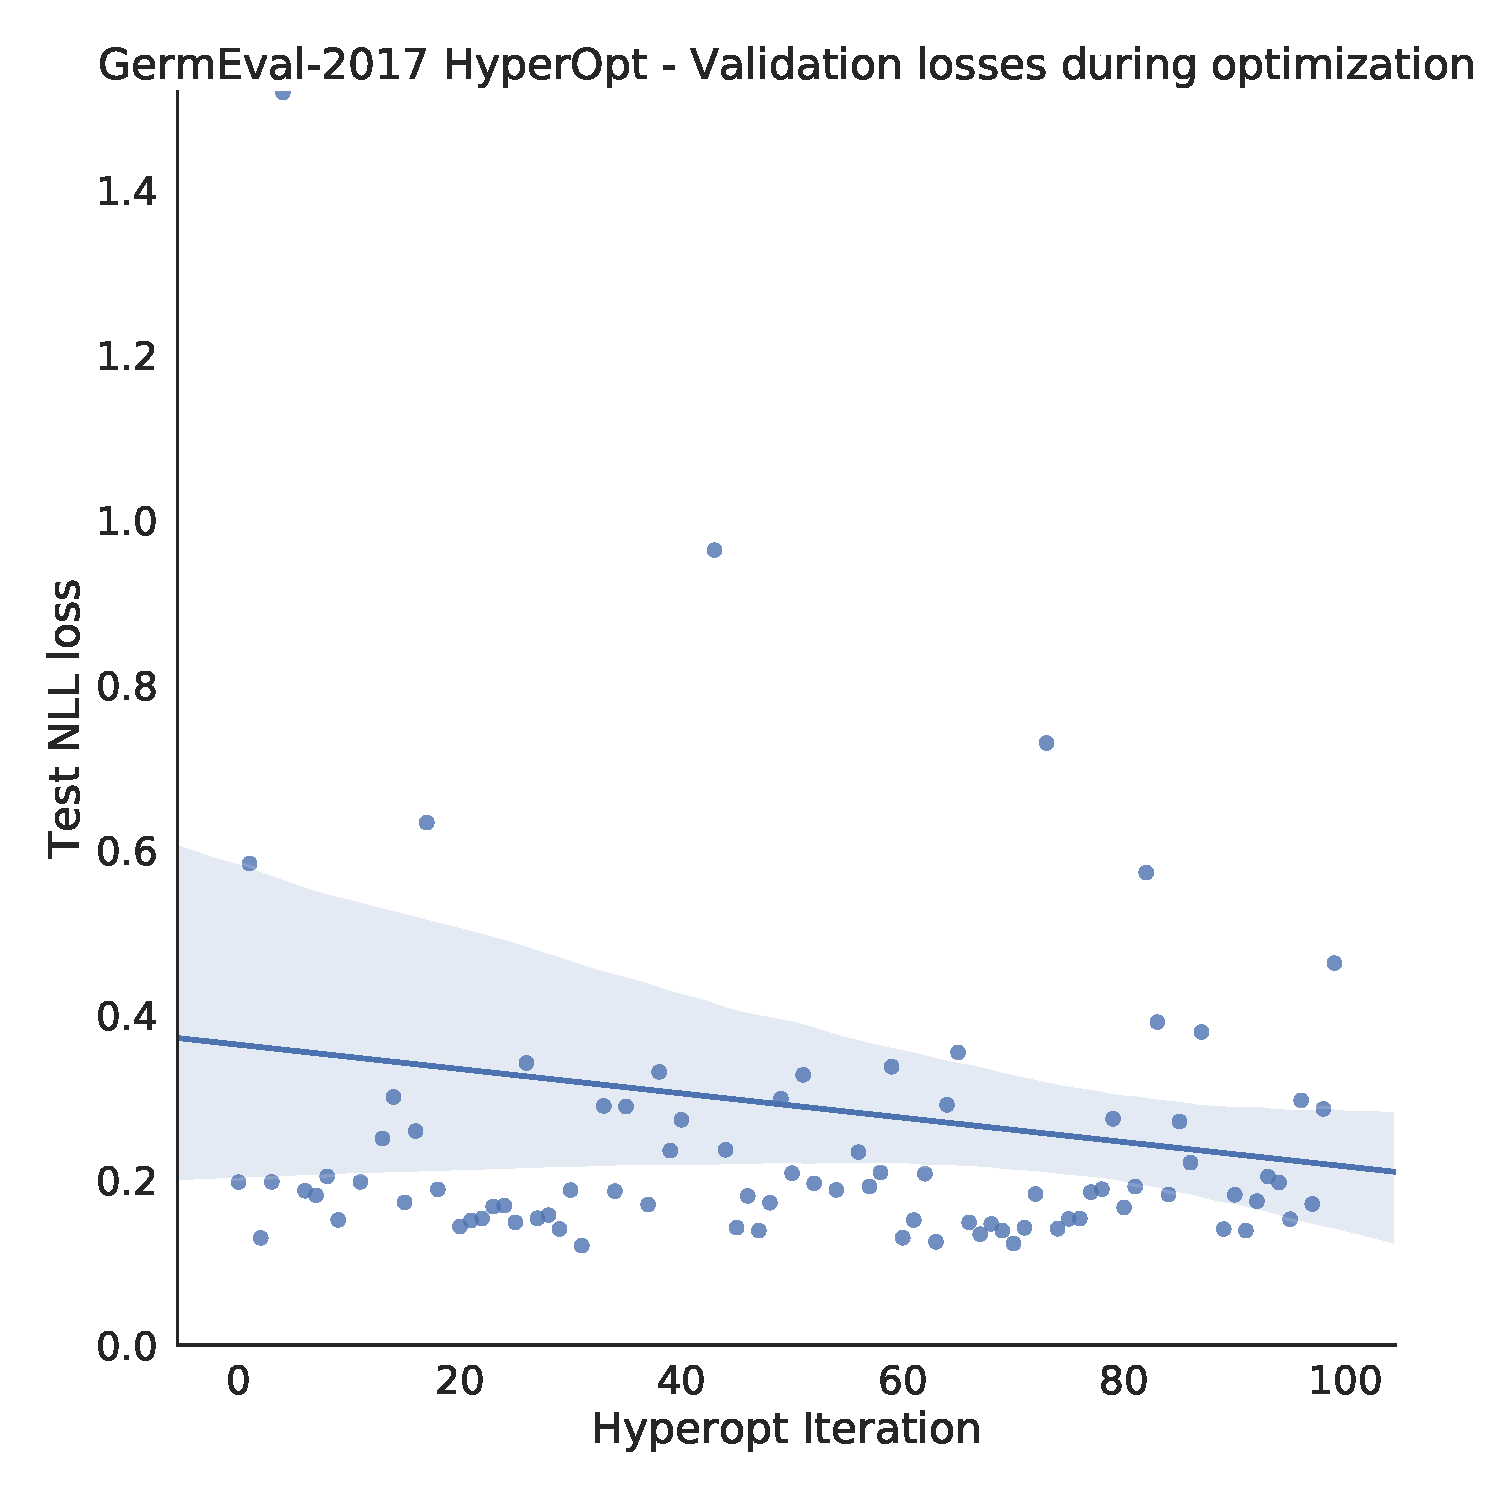
\includegraphics[width=0.49\textwidth]{figures/06_results/06_hp_ge_lm_loss-iteration_validation}
    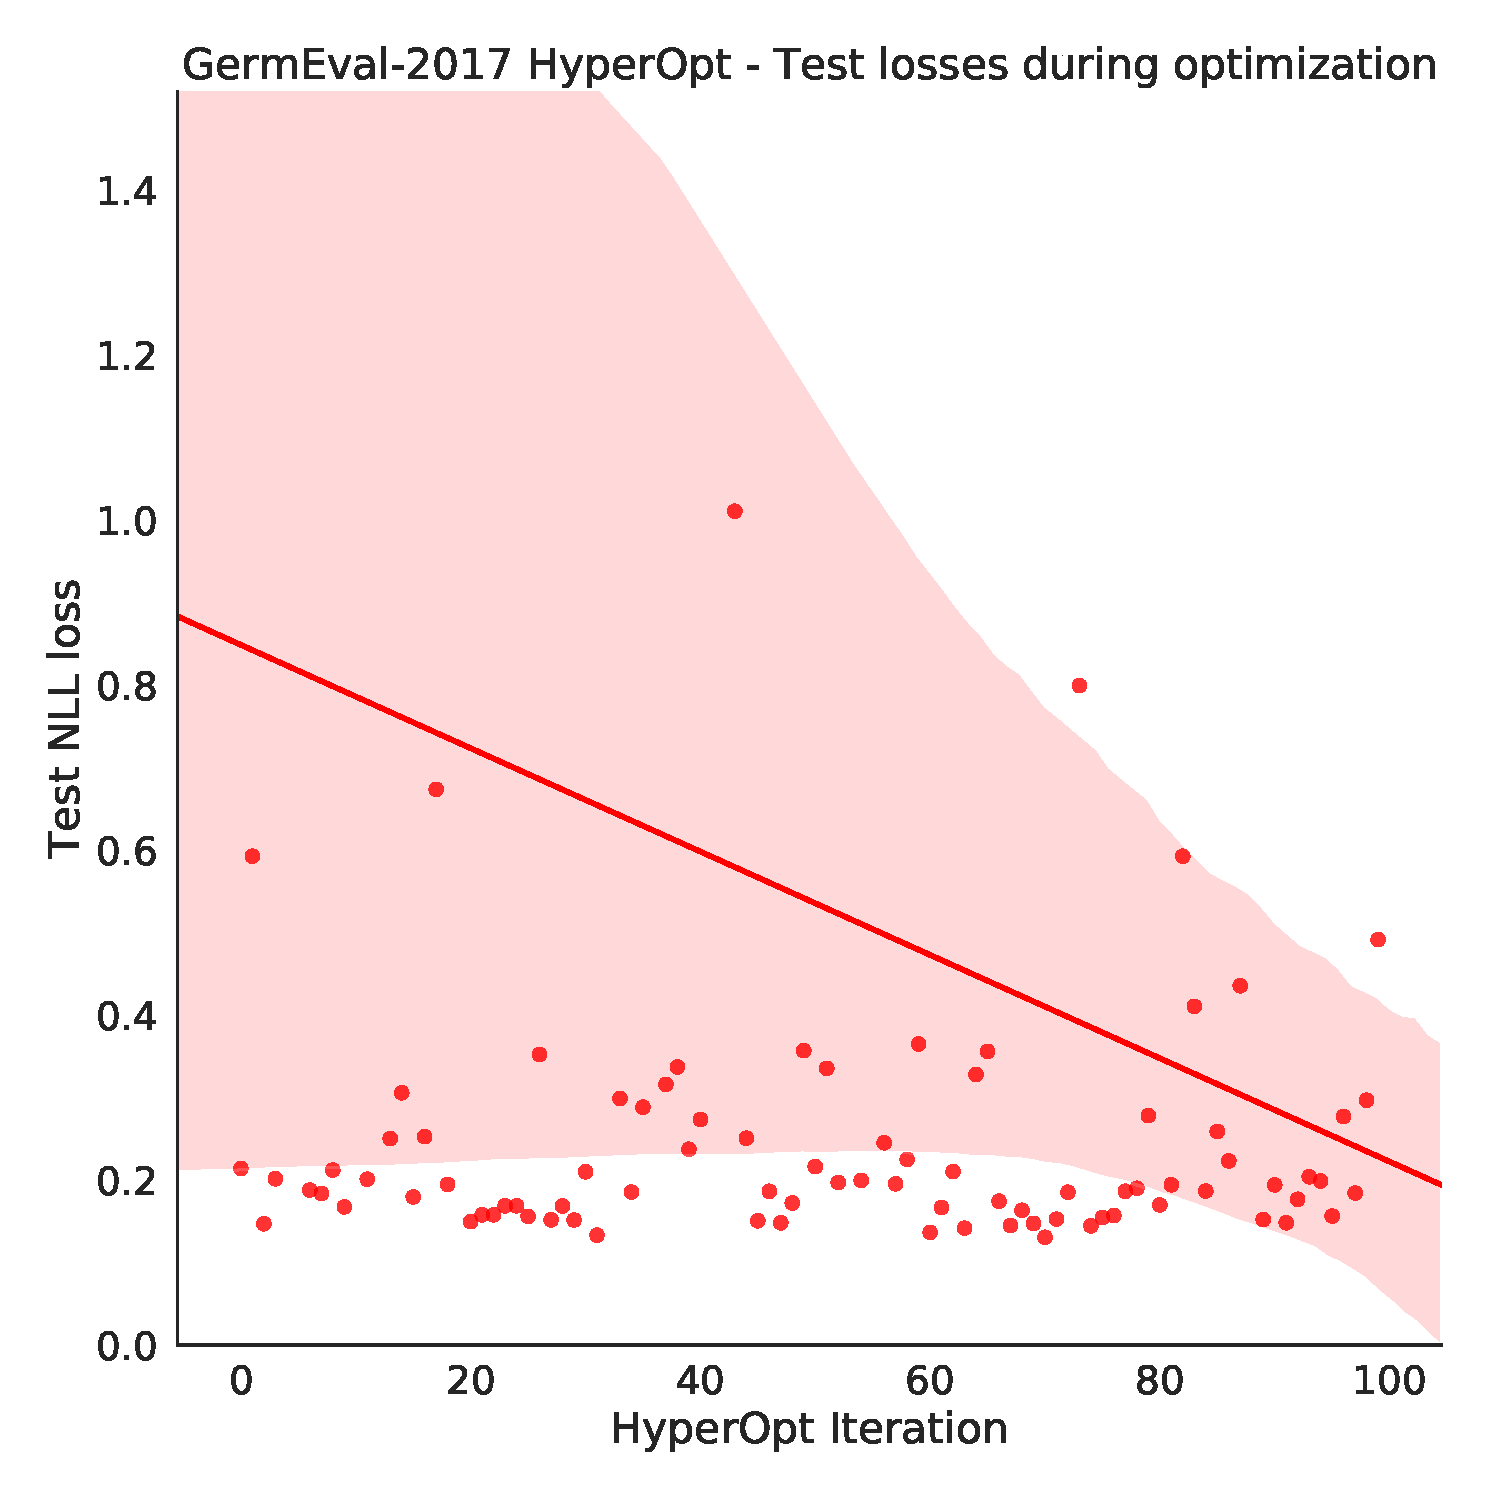
\includegraphics[width=0.49\textwidth]{figures/06_results/06_hp_ge_lm_loss-iteration_test}
    \caption{\textbf{Validation- {(blue -- left)} and test {(red -- right)} losses} during 100 Hyperopt iterations on GermEval-2017 dataset}
    \label{fig:06_ValidationLossGermEvalHp}
\end{figure}

To evaluate Hyperopt three evaluation runs with 100 iterations were performed.

\begin{enumerate}
    \item GermEval-2017 -- \gls{tpe} on validation loss
    \item GermEval-2017 -- Random search
    \item Organic Coarse Grained -- \gls{tpe} on validation loss
\end{enumerate}

Figure~\ref{fig:06_ValidationLossGermEvalHp} visualizes the improvement of the validation- and test losses on the GermEval-2017 dataset after 100 Hyperopt iterations. It seems as if the regression line is negative in both cases which means that the \gls{tpe} algorithm Hyperopt uses suggests better results as the time moves on.

Unfortunately, the \gls{ols} analysis~\ref{tab:08_olsLossItVal} and~\ref{tab:08_olsLossItTest} in the appendix show that the negative correlation is in fact not significant. This analysis implies that the \gls{tpe} algorithm does not sample parameters from the space which improve the loss of the model. This assumption is even more obvious in figure~\ref{fig:06_F1GermEvalHp}. This figure shows the development of F1-Score during optimization. While the results on the left for GermEval might look like they improve throughout the optimization the results\footnote{The improvement is still not significant {(0.340)}} for the optimization of the coarse organic dataset clearly show no improvement.
\medskip

There are several possible explanations which could contribute to this behavior:

\begin{figure}[ht]
    \centering
    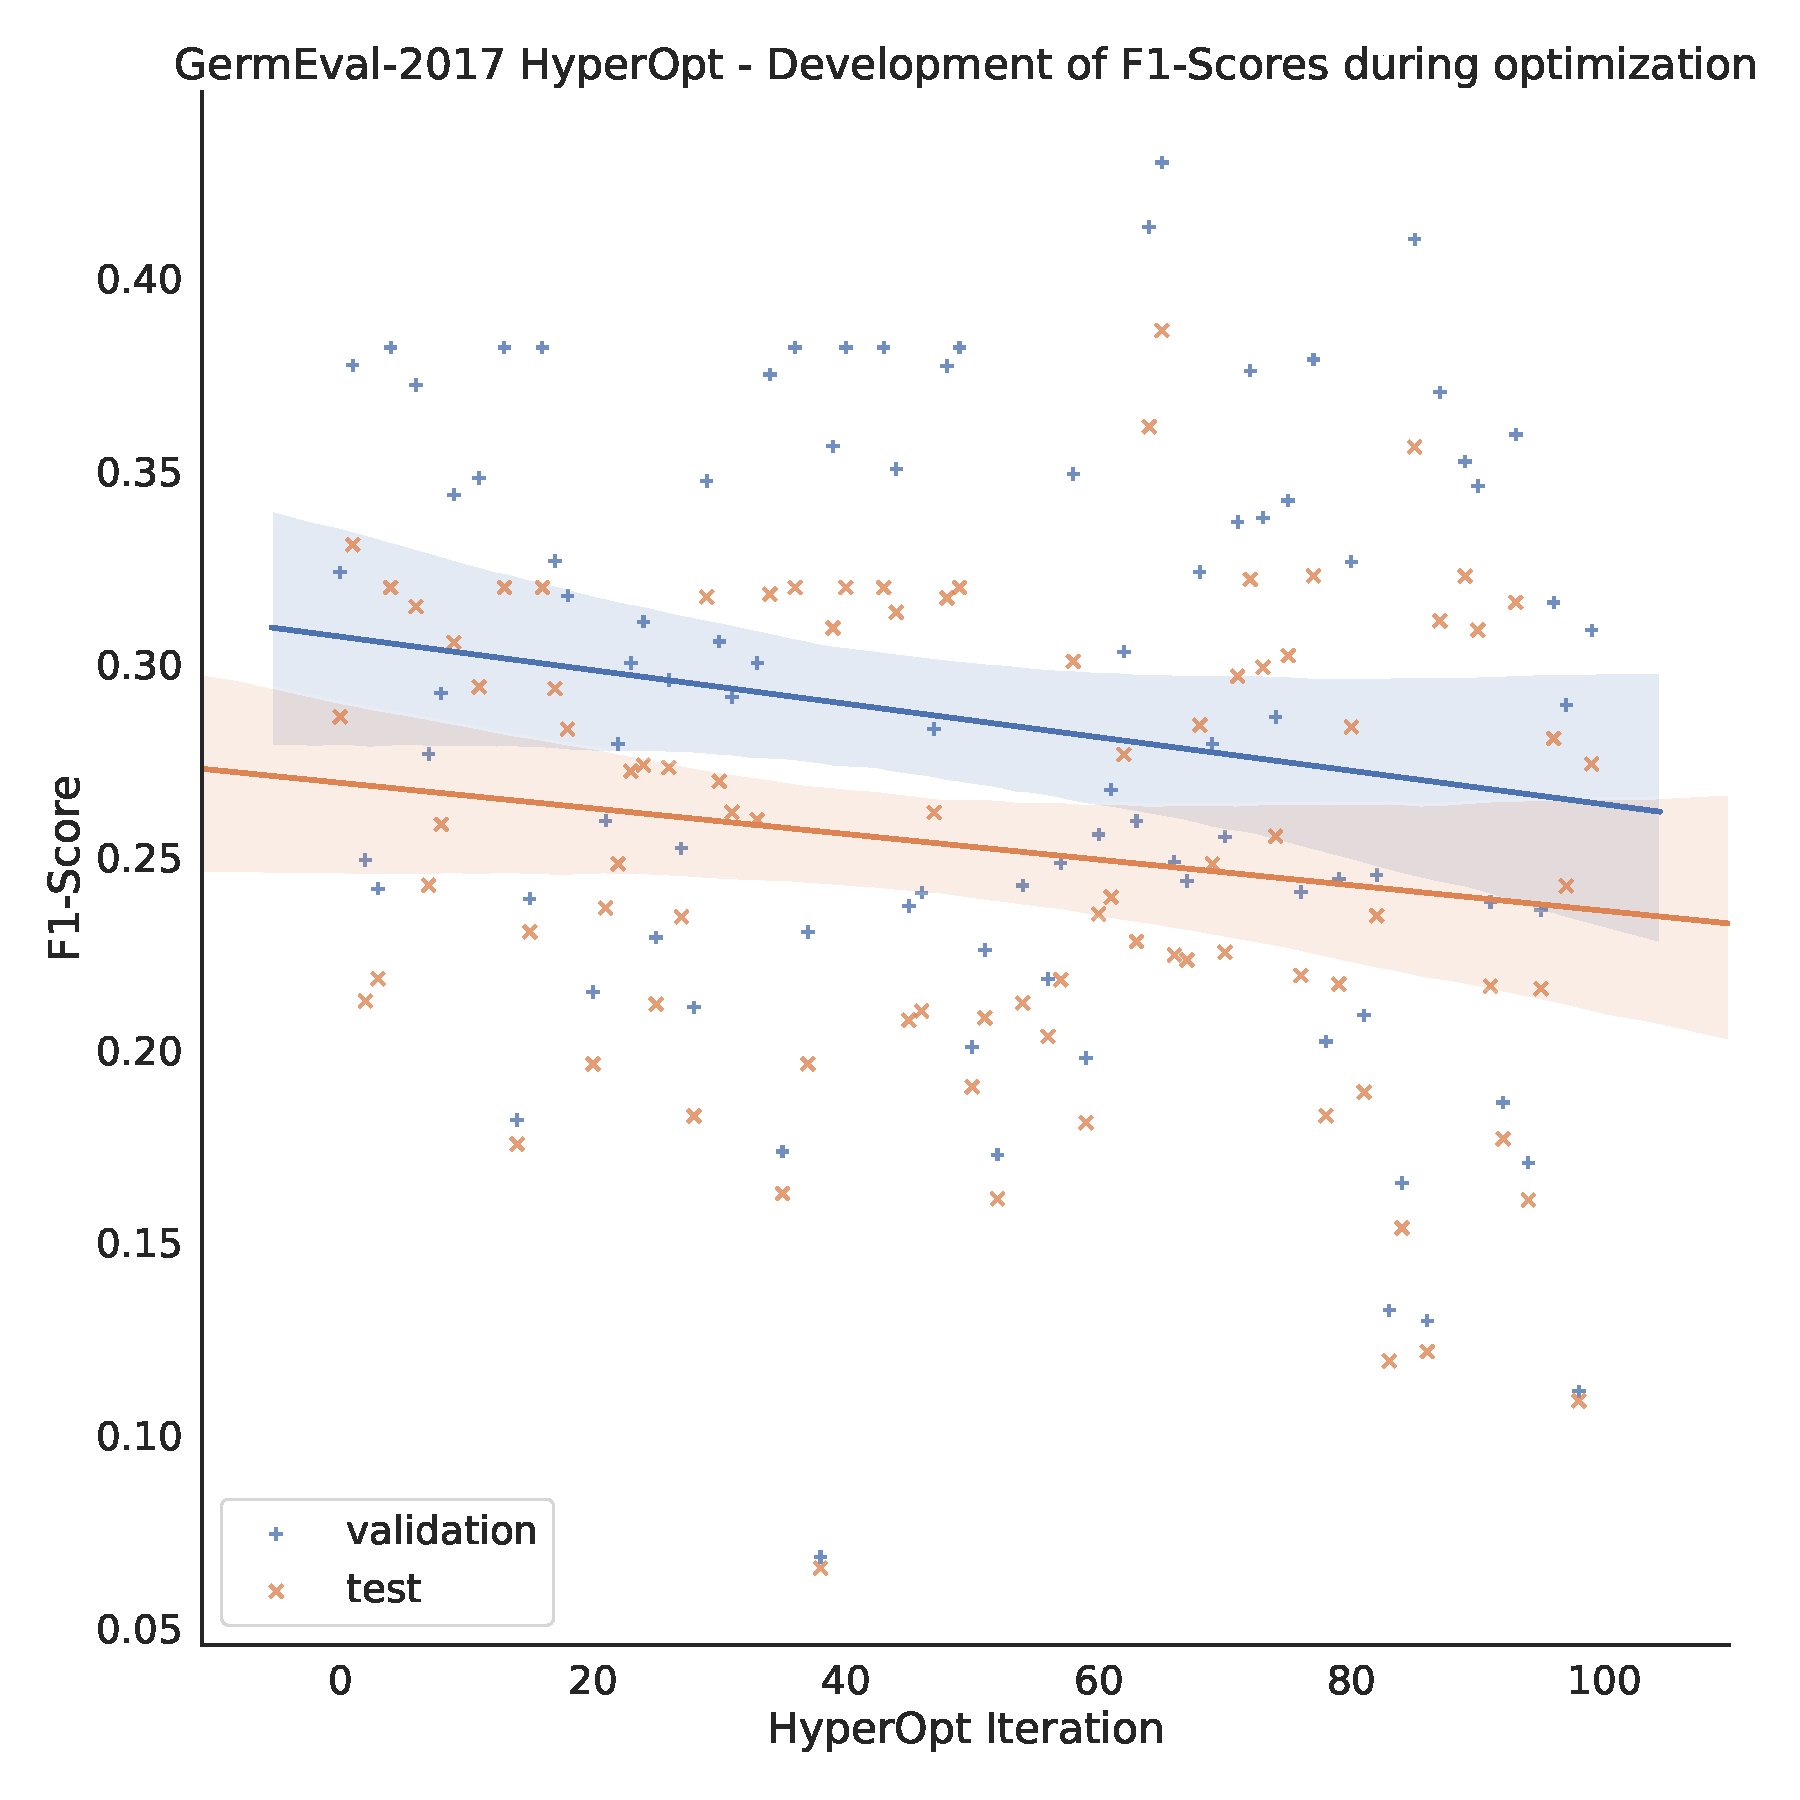
\includegraphics[width=0.49\textwidth]{figures/06_results/06_hp_ge_lm_f1time}
    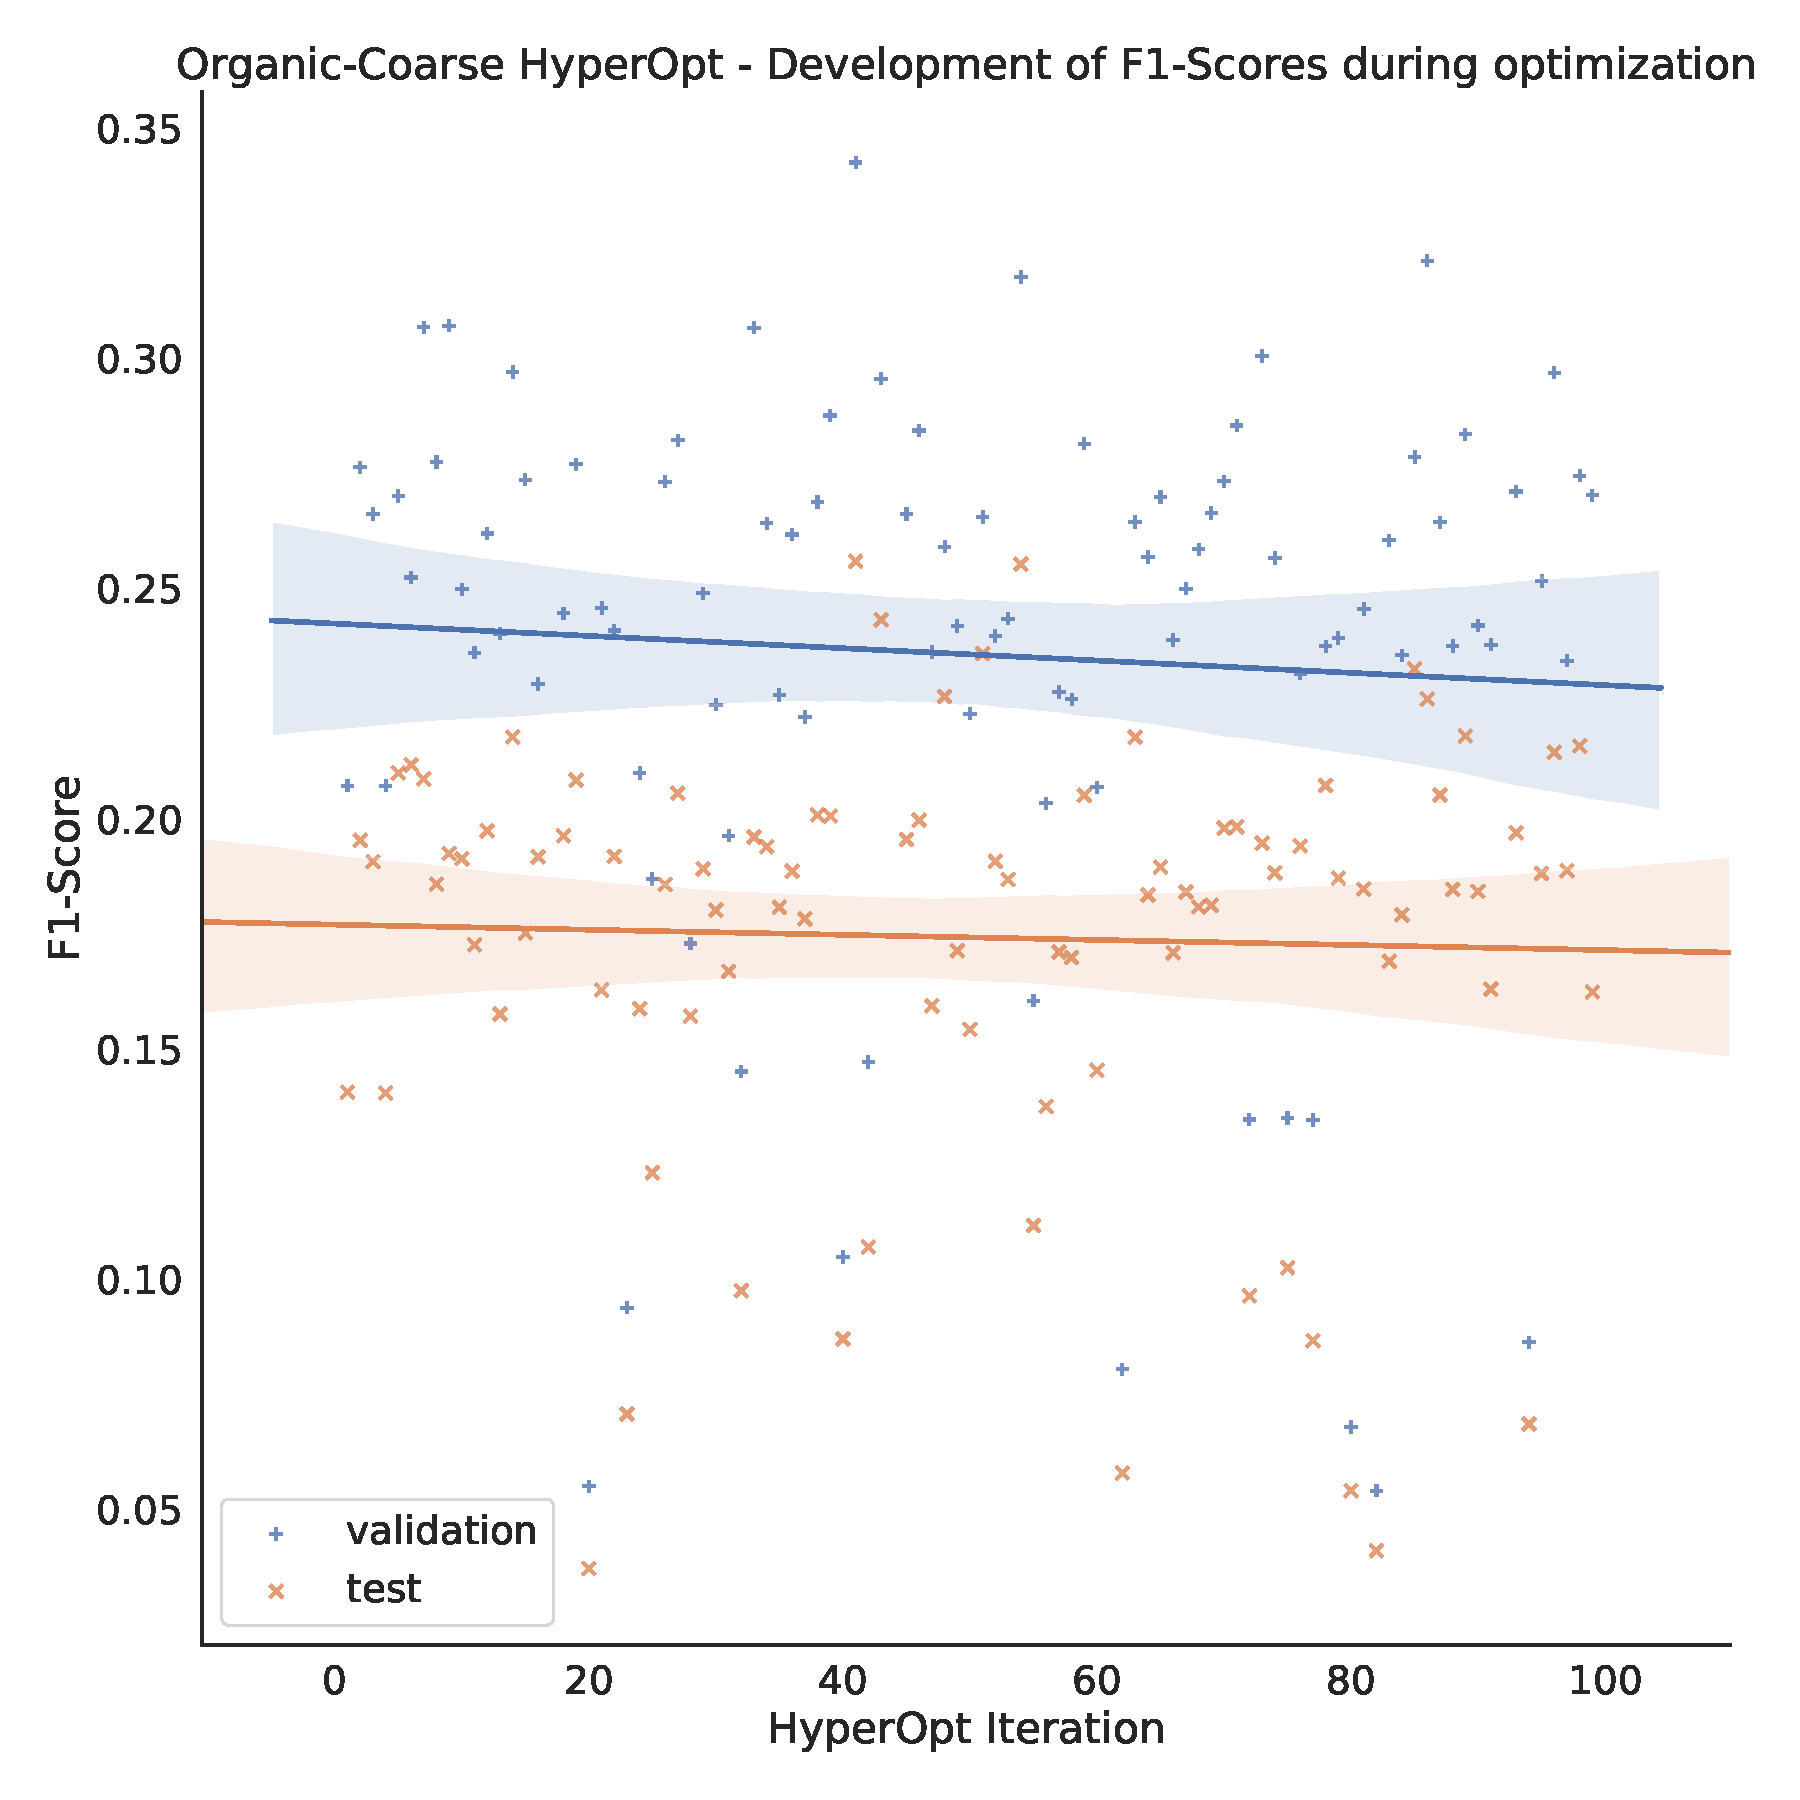
\includegraphics[width=0.49\textwidth]{figures/06_results/06_hp_og_lm_f1time}
    \caption{\textbf{F1 Scores of the hyperparameter optimization} of GermEval-2017 {(left)} and Coarse Organic 2019 datasets {(right)}.}
    \label{fig:06_F1GermEvalHp}
\end{figure}

\subsubsection*{Iterations}

First, it could be possible that 100 iterations are not enough to provide a stochastic model which is able to make good predictions in the hyperparameter space. It is worth noting that Bergstra et al. show that hyperopt outperforms random search within 200 trials~\cite{Bergstra2013}. However, for most architectures, it is not feasible to run an optimization search for much longer than 200 iterations let alone the 1000 iterations they claim as the point where hyperopt converges. 
\medskip

It is also worth mentioning that the Hyperopt module uses a random sampler for the first 10 iterations to get data points to initialize the \glspl{tpe}. Decreasing this number could yield better results for computationally expensive models since the algorithm is forced to suggest values earlier.

\subsubsection*{Hyperparameter Search Space}

It is possible that the hyperparameter search space which Hyperopt uses to generate new parameters is too large. Table~\ref{tab:08_hpSpace} shows the hyperparameter search space for the optimization of the GermEval-2017 dataset. There are parameters which do not change the outcome by a huge margin, and then there are parameters which decide whether or not the model trains at all. However, finding those parameters is a challenging task.

\subsubsection*{Warmup Phase}
\label{sec:06_hp_warmup}
\begin{table}[]
    \centering
    \begin{tabular}{lrrrrr}
    \multicolumn{6}{c}{GermEval-2017} \\

    \toprule
    {} &  count &      mean &       std &       min &       max \\
    Aspect Head &        &           &           &           &           \\
    \midrule
    \multicolumn{6}{c}{Warmup Iterations 1 -- 10*} \\
    CNN-A    &    6 &  0.267644 &  0.050316 &  0.212655 &  0.330922 \\
    MLS-A    &    3 &  0.294608 &  0.032134 &  0.258432 &  0.319838 \\
    \midrule
    \multicolumn{6}{c}{\gls{tpe} Iterations 1 -- 100} \\
    CNN-A    &   67 &  0.249094 &  0.066835 &  0.065565 &  0.386465 \\
    MLS-A    &   23 &  0.261533 &  0.044603 &  0.181078 &  0.356296 \\
    \bottomrule
    \end{tabular}
    \caption{\textbf{Result of sampling of Aspect Head choices during \gls{tpe} Hyperopt optimization.} Values show micro F1-score achieved by models on the GermEval-2017 dataset. * The 10th iteration failed which is the reason why the warmup does not sum up to 10.}
    \label{tab:08_hpAspectHeadsSpace}    
\end{table}

\gls{tpe} supports tree structures for the search space. In the search space used for the optimization, there is one tree-like parameter which is the choice of the aspect head architecture. \gls{tpe} can either choose a \gls{mlsa} or a \gls{cnna}. The \gls{mlsa} does not have additional parameter nodes, whereas the \gls{cnna} has 4 additional parameters.
\medskip

\gls{mlsa} has a higher mean F1-score of 0.263 compared to \gls{cnna} which achieves 0.250. Despite the higher mean score, \gls{tpe} only sampled \gls{mlsa} 23 times compared to 67 times.

This sampling behavior becomes even more interesting when looking at the \gls{tpe} warmup phase. During warmup, \gls{mlsa} is chosen 3 times and \gls{cnna} is chosen 6 times. This ratio is roughly the same distribution compared to the later \gls{tpe} iterations. 

For greater detail refer to table~\ref{tab:08_hpAspectHeadsSpace}. There is also a violinplot which visualizes the impact of the aspect head choice in the appendix as figure~\ref{fig:06_ge_aspectHeadChoices}.
\medskip

In contrast, during the warmup phase of the hyperopt run on the coarse organic dataset, Hyperopt sampled \gls{cnna} 2 times and \gls{mlsa} 7 times which is exactly the other way around. During the \gls{tpe} iterations, \gls{cnna} was sampled 14- and \gls{mlsa} 71 times. Again, this is the exact opposite of the previous optimization on the GermEval-2017 dataset.
\medskip

This behavior leads to the following conclusion: During the warmup phase of hyperopt the search space is randomly sampled. This random sampling distribution is adhered to during the whole \gls{tpe} suggestion phase. This action leads to results which are heavily dependent on the first 10 random iterations.

\subsubsection*{Comparison with a Random Search}

\begin{figure}[ht]
    \centering
    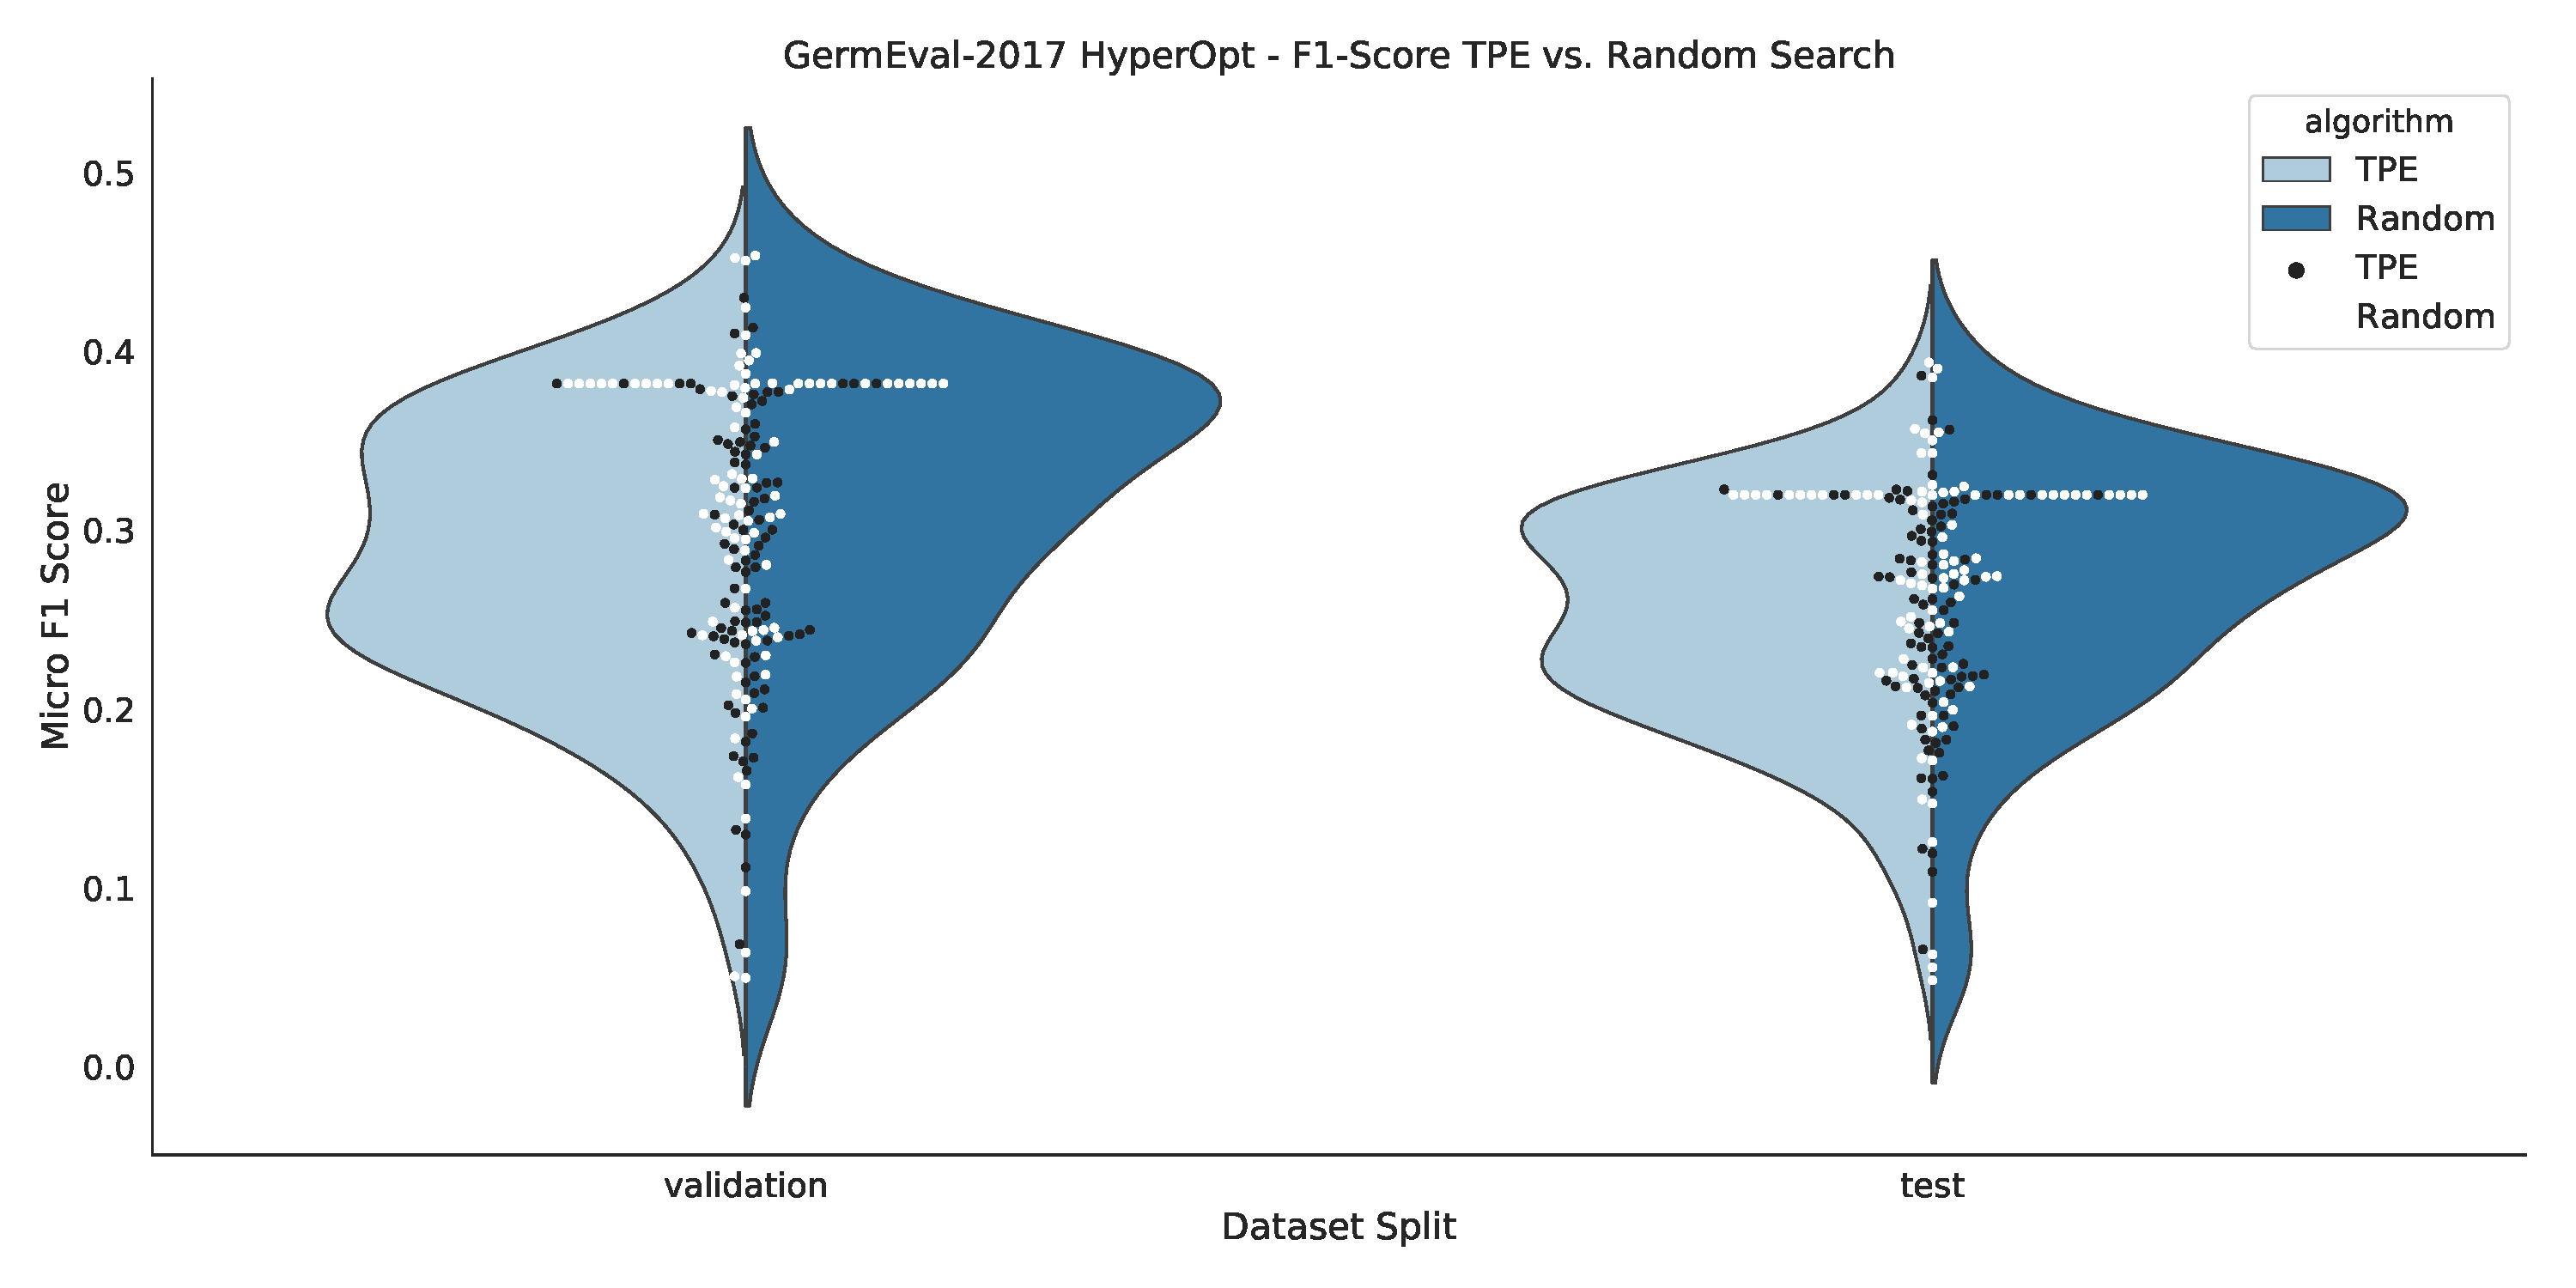
\includegraphics[width=\textwidth]{figures/06_results/06_hp_ge_vio_tpeRand}
    \caption{\textbf{Comparison of HyperOpt TPE algorithm against a classical random search.} The results for TPE are light blue on the left, whereas results for the random search are a deep blue on the right.}
    \label{fig:06_HpOptimTpe_Rand}
\end{figure}

To confirm the findings above a completely random search was performed by Hyperopt on the same number of iterations. The result of this comparison is plotted in figure~\ref{fig:06_HpOptimTpe_Rand}. This violin plot visualizes the result of both optimization runs. The light blue density curve on the left shows the F1 scores from the \gls{tpe} generated models. A broader body on the density curve means that more observations for this particular score value were recorded at this part. The black dots correspond to the actual individual F1-Score observations. The dark blue parts and the white dots correspond to the F1-scores which originated by randomly generated hyperparameters.

\subsection{Model Parameters}

Due to the high dimensionality of the hyperparameter search space, statistical significance tests do not show any significant correlations between the parameter and improvements of the F1-Score. For each single parameter change, all other parameters also change, and they influence the model as well. While not possible to evaluate the results with statistical significance it is possible to derive certain assumptions from the data which are discussed in the following sections.

\subsubsection{Aspect Heads}

As discussed in Section~\ref{sec:06_hp_warmup} it is not entirely possible to favor one or the other aspect head. Both can provide similar results. 

\begin{figure}[ht]
    \centering
    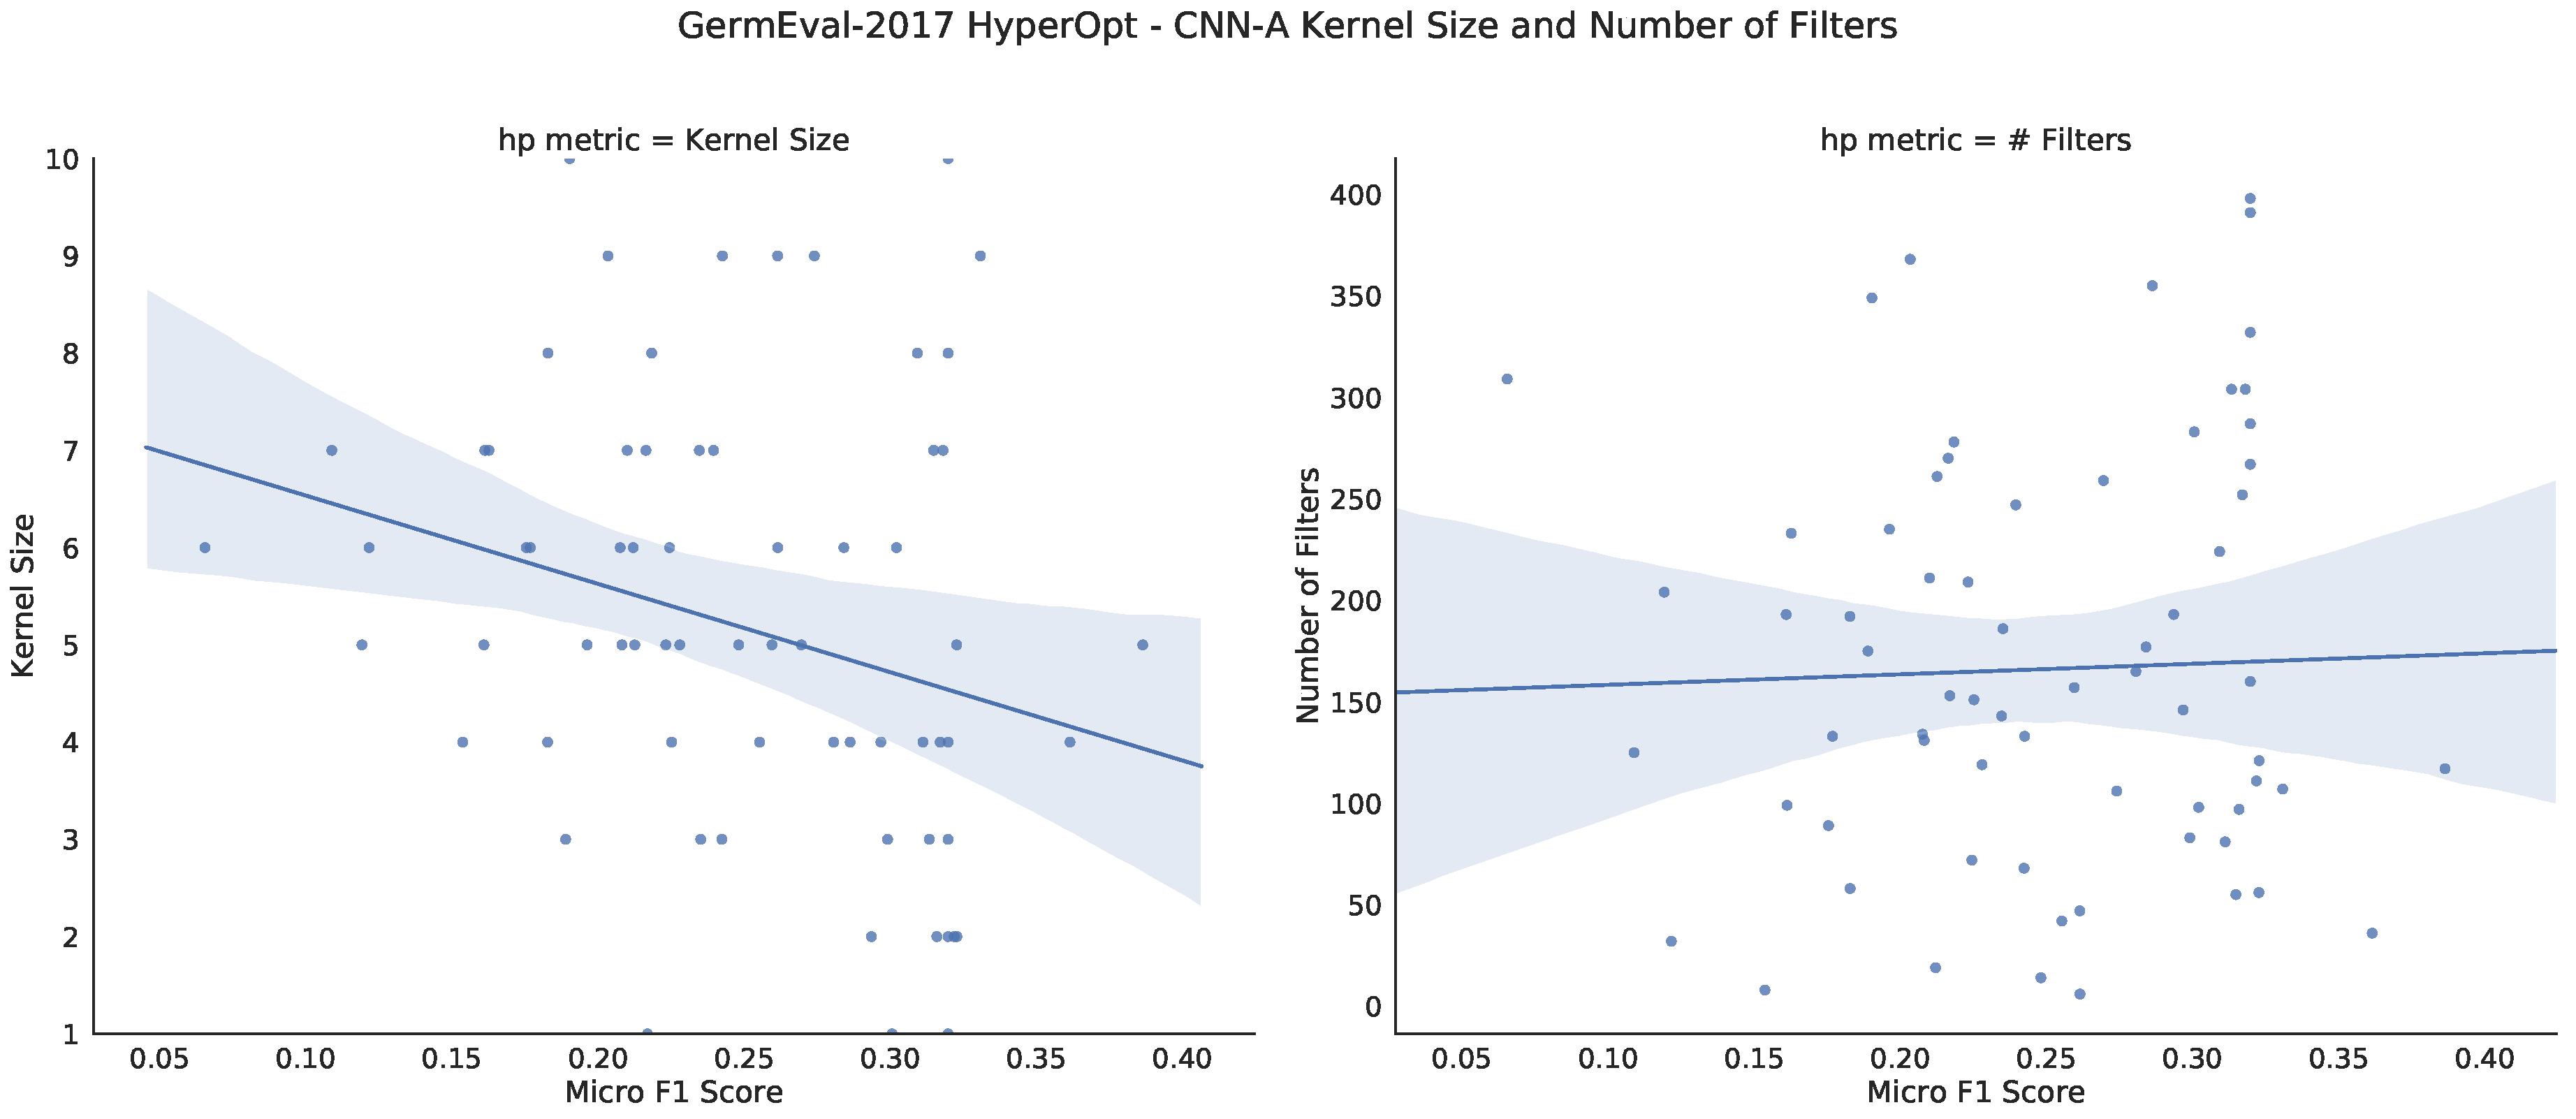
\includegraphics[width=\textwidth]{figures/06_results/06_hp_ge_lm_cnnParams_test}
    \caption{Impact of CNN parameters on micro F1-score. The graph on the left shows the impact of the kernel size on the model performance. The graph on the right depicts the influence of the number of filters on the F1-score.}
    \label{fig:06_HpOptim_CnnParams}
\end{figure}

Figure~\ref{fig:06_HpOptim_CnnParams} shows the impact of the two \gls{cnna} parameters 'Kernel Size' and 'Number of Filters'. The number of filters does not seem to impact the result. However, there is a {(statistical\footnote{Significant at a $p$-value of 0.05})} significant negative correlation between the kernel size and the model performance. 

Smaller filters lead to a performance improvement compared to bigger filters. This result seems to follow the literature. For instance, Schmitt et al. use filter sizes of 3, 4 and 5~\cite{Schmitt2018}.
\medskip

There is no significant change for the other two parameters 'Kernel Padding' and 'Kernel Stride'. The impact on the F1-Score of both parameters is visualized in figure~\ref{fig:06_HpOptim_CnnParams2} in the appendix.

\subsubsection{Point-wise Feed-Forward Layer Size}

In the original transformer model, the inner \acrfull{pwfc} has a dimensionality of 1024 while the model size has a dimensionality of 512~\cite{Vaswani2017c}. This is a 2x increase over the model size. Due to the availability of pre-trained Glove or fastText embeddings our \gls{absat} model only uses a model size of 300. Consequently, the inner \gls{pwfc} layer dimensionality should be around 600. However, layer sizes above 300-400 neurons quickly lead to interesting model behavior. After a few training iterations, the \glspl{pwfc} transform every input to the same output. In other words, no matter what the model gets as input it always predicts the same output.
\medskip

The solution for this overfitting behavior is to use a smaller inner \gls{pwfc}. Values from 100 to 200 neurons lead to the best results.

This is extremely interesting since it completely changes the task of the \glspl{pwfc}. From a layer with a higher dimensionality than the model to a bottleneck layer with lower dimensionality. A larger layer may allow for more complex and expressive features to be learned while a smaller bottleneck layer limits the expressiveness and forces the network to focus on essential features~\cite{Ramsundar2015}.

\subsection{Data Preprocessing}
\label{subsec:06_dataPreprocessing}
In the following section, we discuss the impact of the preprocessing steps and how they affect the overall model performance. 

\begin{figure}
    \centering
    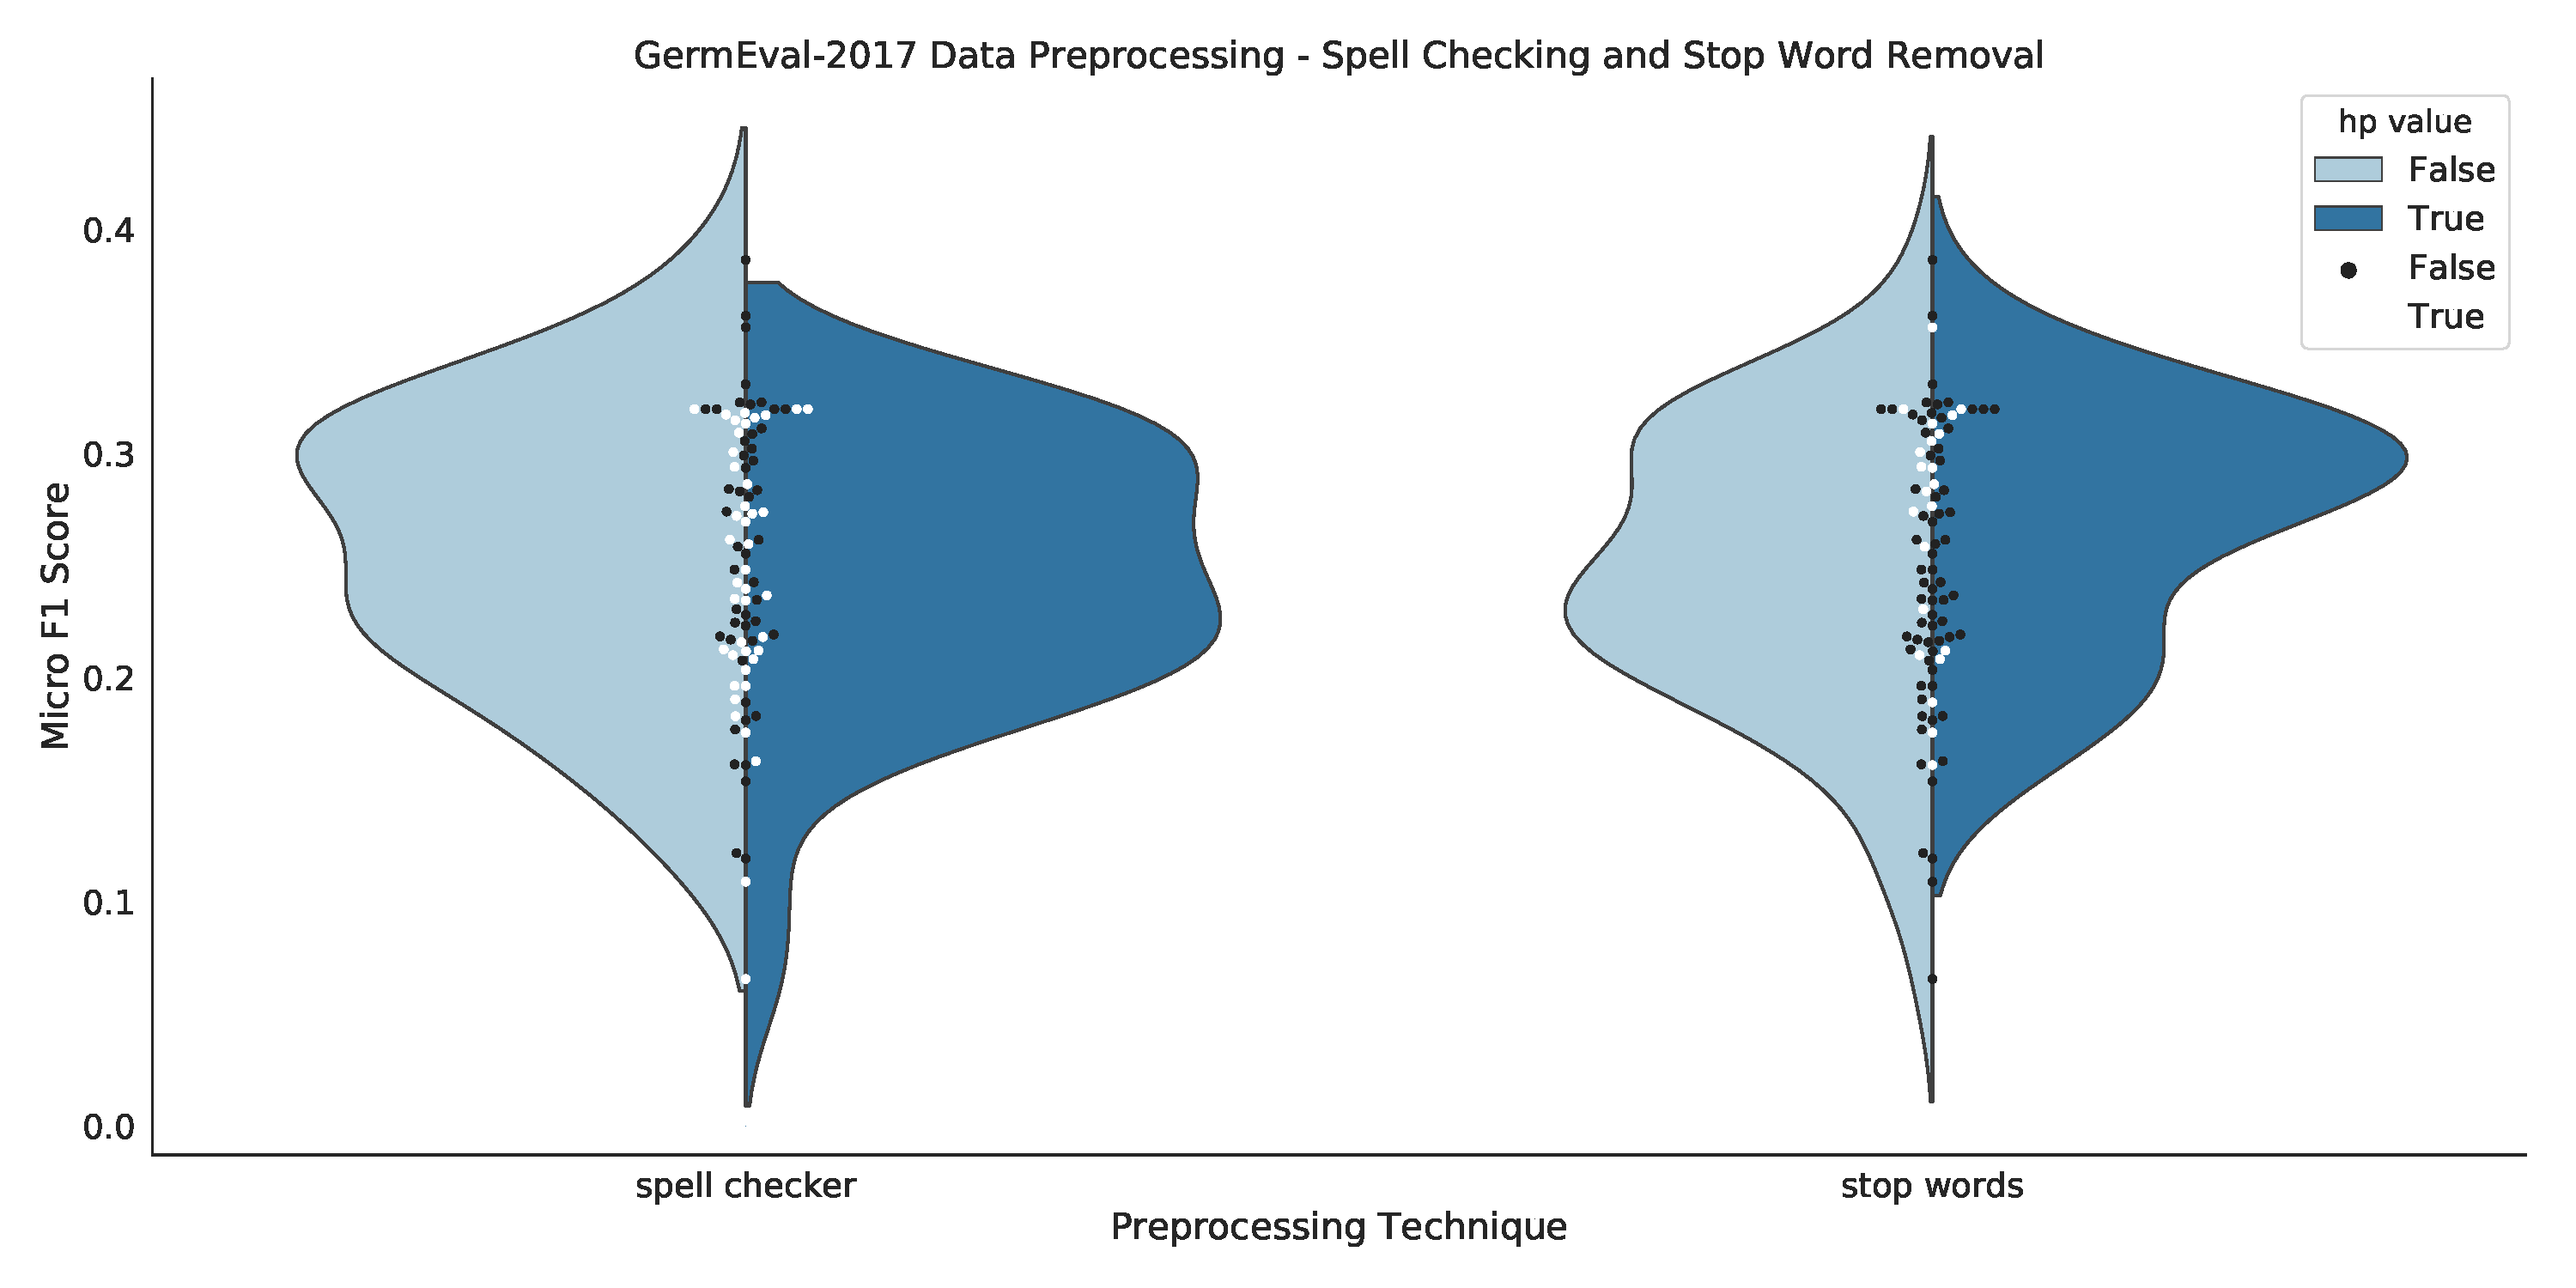
\includegraphics[width=\textwidth]{figures/06_results/06_hp_ge_vio_data}
    \caption{Comparison of preprocessing techniques -- Impact of Spell checking and Stop Word Removal on Validation Micro F1-Score}
    \label{fig:06_PreprocessingHp}
\end{figure}

\subsubsection{Spell Checking}
\label{sec:06_spellChecking}

The left side of figure~\ref{fig:06_PreprocessingHp} shows the impact of spell checking on the GermEval-2017 dataset. In this instance, spell checking negatively impacted the performance of the classifier. There are a few explanations for this performance.
\medskip

Social media content contains a lot of unique characters and words which are not part of a regular dictionary. However, especially those words might carry the most sentiment. By replacing those words, it is possible that a lot of information is lost.
\medskip

Tweets and forums posts about public transport contain a lot of unique abbreviations that spell checkers do not recognize. Persons might be talking about the bad performance of the public transport operator \gls{mvg} but the spell checker replaces 'MVG' with 'mag' {(like)} which changes the sentence dramatically.

\subsubsection{Stop Word Removal}

Stop words are a group of words which are very common in a language but carry little actual information. Examples for stop words are 'the', 'is' or 'what'. The results for stop word removal is shown in figure~\ref{fig:06_PreprocessingHp} on the right side for GermEval-2017. In this specific instance, removing them improves performance. However, this was not as clear for the organic dataset where removing stop words did not significantly improve the performance.

\subsubsection{Comment Clipping}
\label{subsec:06_CommentClipping}

\begin{figure}
    \centering
    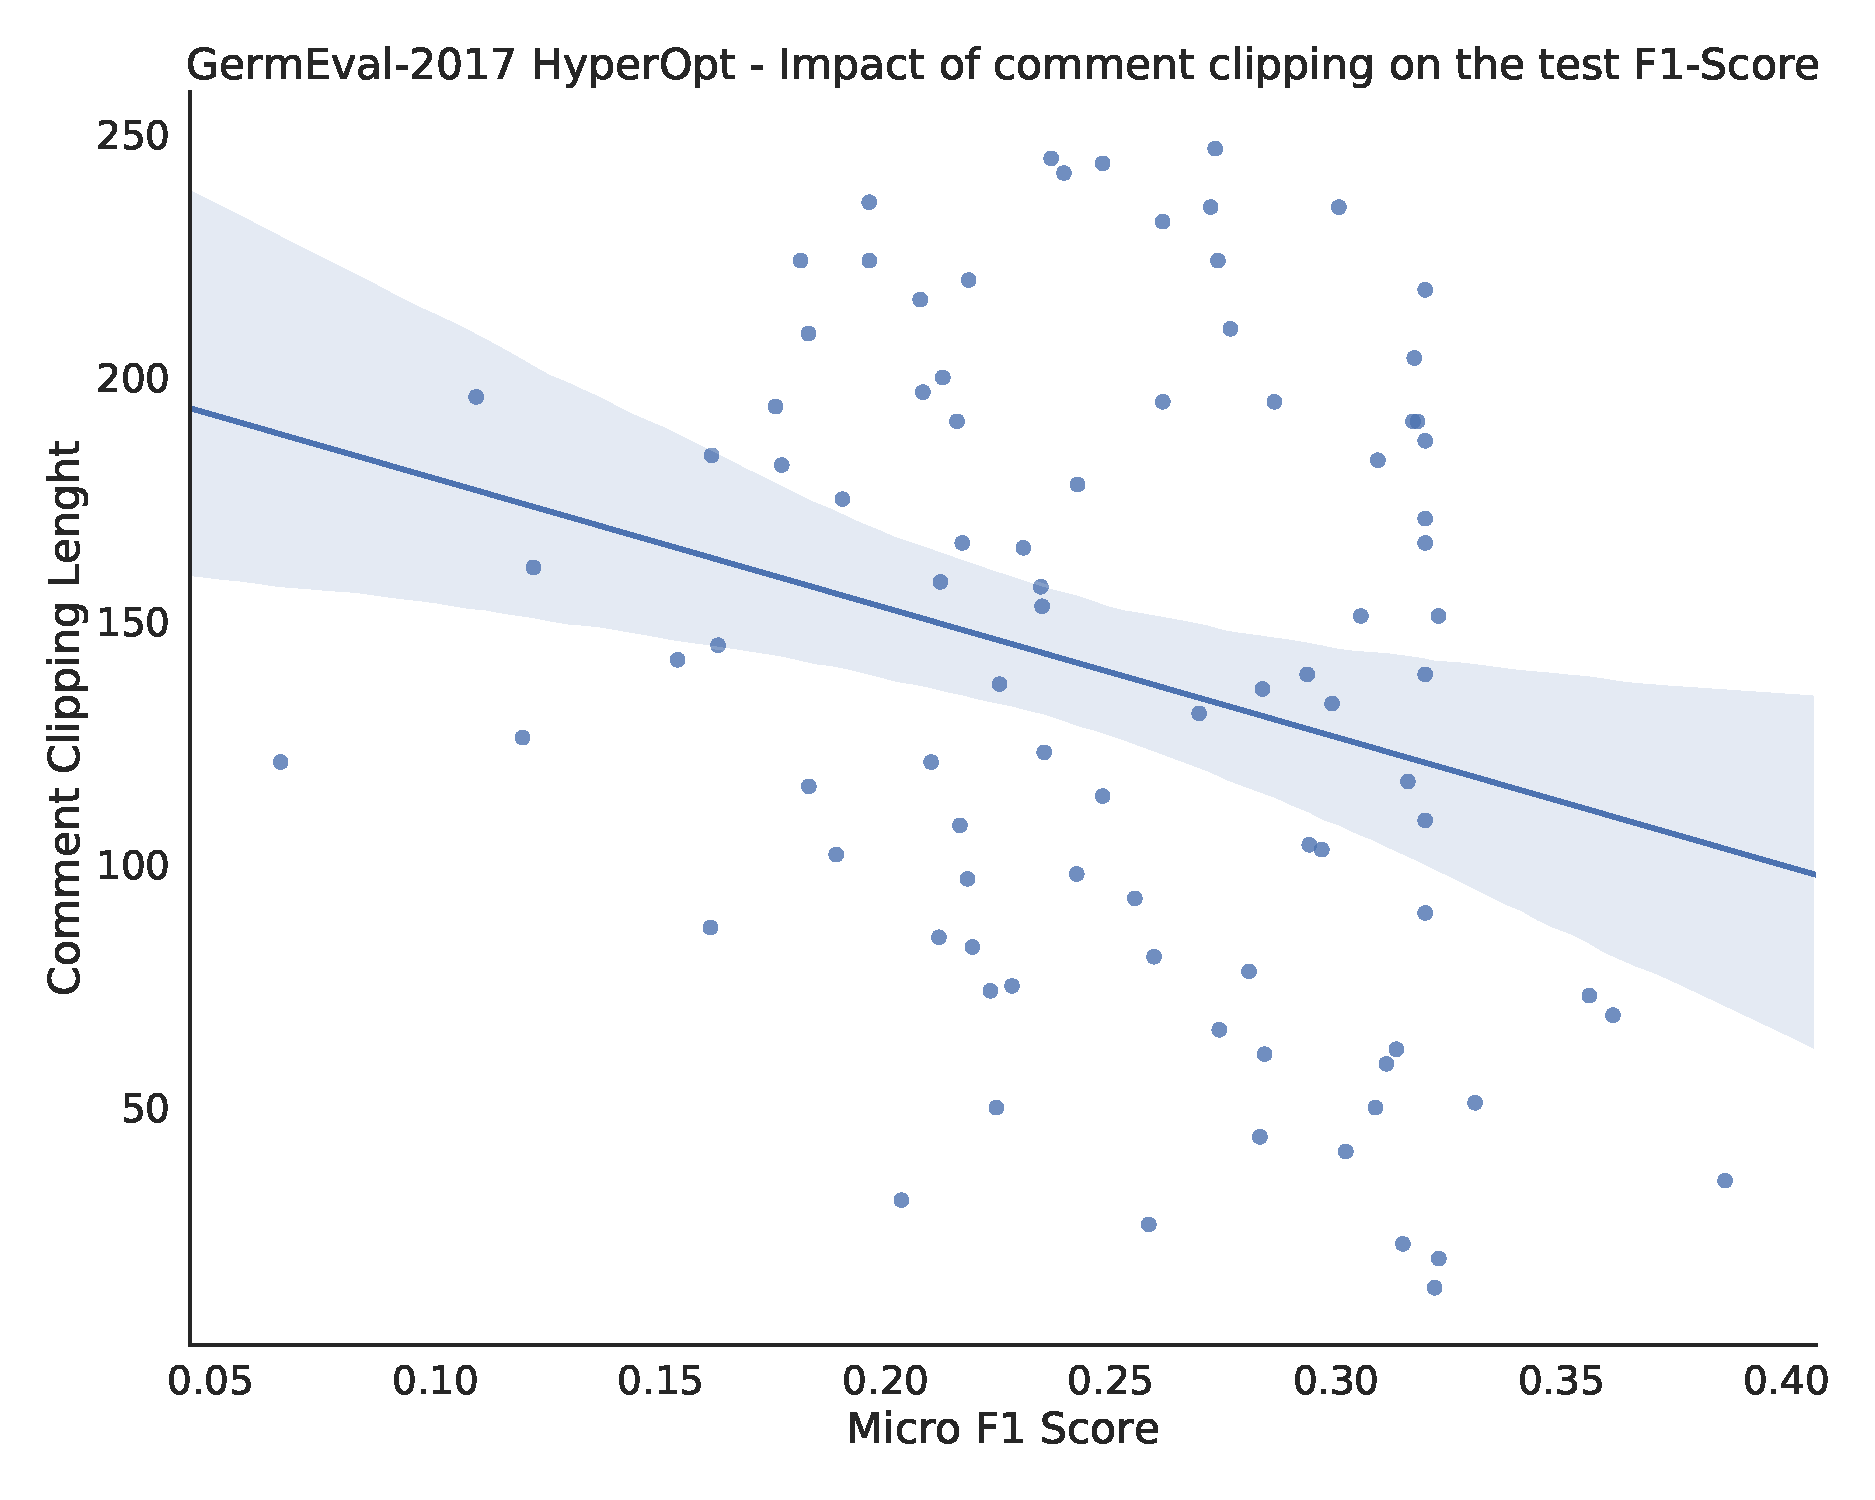
\includegraphics[width=\textwidth]{figures/06_results/06_hp_ge_lm_commentClipping_test}
    \caption{Comparison of preprocessing techniques -- Impact of Comment Clipping on Test Micro F1-Score}
    \label{fig:06_PreprocessingCommentClipping}
\end{figure}

Comment clipping refers to the technique of cutting a sentence or comment after a specific number of tokens. In other words, comments which are too long are shortened, and comments which are too short are padded.

Figure~\ref{fig:06_PreprocessingCommentClipping} provides a visualization how comment clipping impacts the model performance on the GermEval-2017 dataset. The regression line shows that a shorter sequence length may improve performance of the overall model\footnote{Significant at a $p$-value of 0.05}.
\medskip

This observation seems to be reasonable since GermEval-2017 contains a mix of very short tweets {(140/280 character limit)} as well as long newspaper articles. Aligning them to an overall shorter length seems logical especially considering that most longer newspaper articles include a summary in the beginning. Cutting those long documents helps the transformer to focus on relevant information instead of spreading out the attention.

\section{Results for Named Entity Recognition}

The following section contains the final results for the \acrfull{ner} task of the CoNLL-2003 dataset.

Since this task was an auxiliary training task to assess the performance of the transformer part, no hyperparameter tuning was performed.
\medskip

For this dataset, the architecture is slightly different, because CoNLL-2003 has annotations for each word. Since the transformer makes predictions per word, there is no need for separate aspect heads.

Therefore, this architecture follows the original transformer and consists of a single linear layer to project the 300-dimensional per-word prediction down to the number of classes to predict. Finally, a log-softmax is used to provide the log probabilities for the class labels.
\medskip

For the final evaluations, we use a transformer model with two encoder blocks, each consisting of two attention heads. We employ a model dropout rate of 0.3 and a pointwise layer size of 300. Furthermore, we use FastText embeddings a batch size of 12 and a weight decay of $1e^{-6}$.

\begin{table}[]
    \centering
    \begin{tabular*}{\textwidth}{l@{\extracolsep{\fill}}cccc@{}}
    \toprule
    Variant          & \multicolumn{2}{c}{\textbf{Macro F1}}     & \multicolumn{2}{c}{\textbf{Micro F1}}       \\ 
    \midrule
                     & \textit{dev}          & \textit{test}         & \textit{dev}              & \textit{test}         \\
    \midrule
    Random Classifier          &  0.147       & 0.187     &  0.210          &   0.214  \\
    CoNLL-2003 Baseline         &  -            &  -        & -                &   0.596         \\
    CoNLL-2003 Best Result & - & - & - & 0.888 \\
    Baevski et. al 2019 {(\gls{sota})}          & -            & -            & 0.969         &   \textbf{0.935}         \\
    Transformer {(our)}      & 0.822             & 0.766    &  0.939                &   0.918               \\ 
    \bottomrule
    \multicolumn{5}{c}{\textbf{CoNLL-2003 -- NER}} \\
    \end{tabular*}
    \caption{Results of models on the shared CoNLL-2003 task for \gls{ner}. The random classifier acts as a minimal baseline as it will predict completely random classes for each sample. The CoNLL-2003 baseline~\cite{Erik2003} was provided for the CoNLL-2003 NER competition. The best result at the competition achieved an F1-score of 0.8876~\cite{Florian2003}. At the time of writing {(April 2019)}, the best result on CoNLL-2003 NER is achieved by Baevski et al.~\cite{Baevski2019}}.
    \label{tab:06_resultsConLL}
    \end{table}

\bigskip
Table~\ref{tab:06_resultsConLL} lists the result of our and other submissions for this task to assess the fitness of this model. The vanilla transformer model already achieves very competitive results. It outperforms every original submission for CoNLL-2013 by a wide margin and is only slightly behind the current state of the art~\cite{Baevski2019} even though it was not exclusively created for this purpose.
\medskip

\begin{figure}[ht]
    \centering
    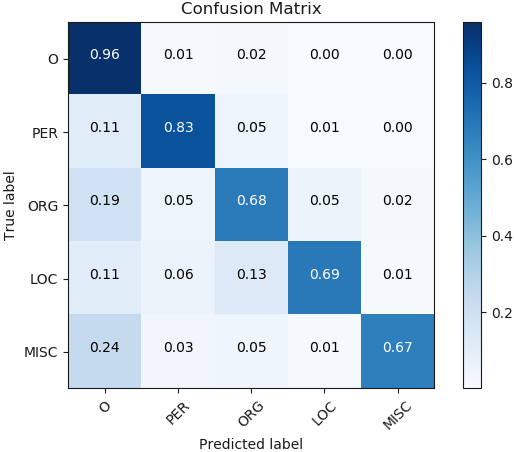
\includegraphics[width=0.49\textwidth]{figures/06_results/06_ner_final_test_c_matrix}
    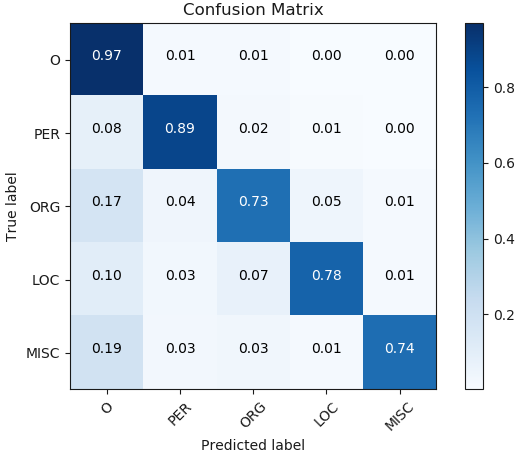
\includegraphics[width=0.49\textwidth]{figures/06_results/06_ner_final_valid_c_matrix}
    \caption{Normalized confusion matrices for the \gls{ner} task of the CoNLL-2003 dataset. The matrix on the left shows the performance of the model on the test set while the right confusion matrix visualizes the performance on the validation / development set.}
    \label{fig:06_NER_cmatrices}
\end{figure}

The normalized confusion matrices in figure~\ref{fig:06_NER_cmatrices} show the performance of the transformer on the dataset for the individual classes. The class 'LOC' is the most frequent class in the dataset {(see table~\ref{tab:05_conll2003DatasetStats})} aside from class 'O' which is the 'Other' class. Despite this fact, the class performed poorly considering the 'MISC' class which achieved a similar result only has half the training samples.



\section{Results for Aspect-Based Sentiment Analysis}
The following sections outline the results of \acrfull{absa}. The first section contains the results for the GermEval-2017 dataset. This dataset uses a unique evaluation method. To be able to compare our results we also use the evaluation method that GermEval-2017 provides.

The method GermEval-2017 uses is described in Section~\ref{sec:05_GermEvalEvaluation}.
\medskip

Section~\ref{sec:06_ResultsOrganic} reports results on the Organic-2019 dataset and Section~\ref{sec:06_ResultsAmazon} discusses the results on the Amazon Reviews dataset.

Finally, Section~\ref{sec:06_ResultsMultitask} and~\ref{sec:06_ResultsTransfer} review the results of multitask learning and transfer learning.

\subsection{Results for GermEval-2017}
\label{sec:06_ResultsGermEval}

\begin{table}[htp]
    \centering
    \begin{tabular*}{\textwidth}{l@{\extracolsep{\fill}}cccc@{}}
    \toprule
    Variant          & \multicolumn{2}{c}{\textbf{Macro F1}}     & \multicolumn{2}{c}{\textbf{Micro F1}}       \\ 
    \midrule
                     & \textit{synchronic test}          & \textit{diachronic test}         & \textit{synchronic test}              & \textit{diachronic test}         \\
    \midrule
                                 \multicolumn{5}{c}{GermEval-2017 competition~\cite{Wojatzki2017}}                     \\
    Majority Baseline                 &  -            &  -        & 0.315            &   0.384                             \\
    \gls{svm} Baseline                 &  -            &  -        & 0.322            &   0.389                             \\
    Best Submission                  &  -             &  -         & 0.354         & 0.401                             \\
    \midrule
                                 \multicolumn{5}{c}{Schmitt et al. 2018 {(\gls{sota})}~\cite{Schmitt2018}}         \\
    Pipeline \gls{lstm} + FT          & -            & -            & 0.297         &   0.342                            \\
    End-to-end \gls{lstm} + FT          & -            & -            & 0.315         &   0.384                             \\
    Pipeline \gls{cnn} + FT          & -            & -            & 0.295         &   0.342                             \\
    End-to-end \gls{cnn} + FT          & -            & -            & \textbf{0.423}&   \textbf{0.465}                     \\
    \midrule
    \multicolumn{5}{c}{Dugar 2019~\cite{Dugar2019}}                                                     \\
    End-to-end \gls{lstm} + FT          & 0.56            & -            &  0.384 &   -                     \\
    \midrule

                                 \multicolumn{5}{c}{Our Results}                                                     \\

    Random Classifier                   &  0.014       & 0.014     &  0.018          &   0.018                              \\
    \gls{absat} + \gls{lmh} + FT     & 0.131        & 0.111        &  0.390        &   0.413                               \\ 
    \gls{absat} + \gls{cnnh} + FT    & 0.102        & -            &  0.352          &   -                               \\ 
    \bottomrule
    \multicolumn{5}{c}{\textbf{GermEval-2017 -- Task C {(ABSA)}}} \\

    \end{tabular*}
    \caption{Evaluation and comparison of models on the shared GermEval-2017 task for \gls{absa}. The random classifier acts as a minimal baseline as it predicts completely random classes for each sample. The organizers of GermEval-2017 provide two baselines~\cite{Wojatzki2017}. The first one, predicts the majority class which is \textit{"Neutral-Allgemein"}. This baseline already achieves a score of 0.315 on the synchronic test set. The second baseline uses a \gls{svm} classifier and achieves strong results of 0.322 and 0.389. The best submission for the GermEval-2017 challenge was achieved by Lee et al.~\cite{Lee2017} with a score of 0.355 and 0.401. Schmitt et al. achieved \gls{sota} in 2018 with an End-to-end \gls{cnn} model with custom FastText {(FT)} embeddings. Their best score is 0.423 on the synchronic- and 0.465 on the diachronic test set. Our \gls{absat} model with linear mean heads and FastText embeddings outperforms every submission of the GermEval-2017 competition and is competitive with the end-to-end \gls{cnn} model of Schmitt et al.}
    \label{tab:06_resultsGermEval}
\end{table}

The GermEval-2017 dataset for \acrfull{absa} is a large dataset for multi-label aspect sentiment detection. In addition, it is reasonably closely related to the Organic-2019 dataset which is the reason why this dataset was used to evaluate the model. Both datasets use posts form social media. Therefore, the task of detecting aspect-based sentiment is similar. This dataset is also much larger than Sem-Eval-14, -15 or -16.
\medskip

Furthermore, Schmitt et al. -- one of the inspirations for this thesis -- use GermEval to evaluate their model. To compare the base transformer model we used the CoNLL-2003 NER task. To compare the whole architecture against other approaches, it makes sense to use GermEval since there are other results which we can use to compare the performance of the \acrfull{absat} model.
\bigskip

Table~\ref{tab:06_resultsGermEval} reports on the result of the evaluation of our \gls{absat} against other GermEval models. The first three results are models created for the GermEval-2017 competition. Wojatzki et al. provide two baseline systems for the \gls{absa} task~\cite{Wojatzki2017}. The first one is a majority class baseline which predicts the class which contains most samples. For this dataset, this is the class "Allgemein -- Neutral". 
\medskip

Since GermEval is very skewed towards this majority class the baseline is very strong. Refer to figure~\ref{fig:08_germEvalStatistics} for an overview of the aspects and their distributions. The second baseline system is a \gls{svm} classifier. At the time of the competition, this baseline was very competitive and achieved second place. Finally, the best submission for GermEval-2017 by Lee et al. achieves a micro F1 score of 0.354 on the first test set {(synchronic test)} and 0.401 on the second test set {(diachronic test)}.
\medskip

The current \acrfull{sota} is an end-to-end \gls{cnn} architecture by Schmitt et al.~\cite{Schmitt2018} with custom FastText Embeddings. This architecture achieved a micro F1 score of 0.423 on the synchronic test set and 0.465 on the diachronic test set. 
\medskip

In comparison, our \gls{absat} model accomplishes a micro F1 score of 0.390 and 0.413 on the first and second test sets. This result means that our model outperforms even the best submission for the GermEval-2017 competition. In addition, the \gls{absat} model with \glspl{lmh} is competitive with the end-to-end \gls{cnn} created by Schmitt et al.
\medskip

Several techniques can be applied to produce even better results for the task. Schmitt et al. show that pre-training custom FastText embeddings on the target domain improve the model. Dugar also demonstrates that data augmentation can positively impact model performance~\cite{Dugar2019}. 
\smallskip
In Section~\ref{sec:06_ResultsTransfer} we also demonstrate, that transfer learning positively impacts model performance. However, finding similar data in German might be challenging.

\subsection{Results for Amazon Product Reviews}
\label{sec:06_ResultsAmazon}

\begin{table}[htb]
    \centering
    \begin{tabular*}{\textwidth}{l@{\extracolsep{\fill}}ccccc@{}}
    \toprule
    Variant          & \multicolumn{2}{c}{\textbf{Macro F1}}     & \multicolumn{2}{c}{\textbf{Micro F1}} &       \\ 
    \midrule
                     & \textit{dev}          & \textit{test}         & \textit{dev}              & \textit{test} & Train Duration        \\
    \midrule
    Random Classifier                      &  0.031        & 0.031      &  0.031        &   0.031    & -        \\
    \gls{absat} + \gls{lmh} + FT + SP   & 0.461         & 0.513        &  0.461        &   0.513   & 49h            \\ 
    \bottomrule
    \multicolumn{6}{c}{\textbf{Amazon Reviews Dataset}} \\
    \end{tabular*}
    \caption{Results of the \gls{absat} model with mean linear aspect heads {(LMH)} and FastText {(FT)} embeddings on the custom amazon reviews dataset. Spell checking {(SP)} is enabled. The model reported in this table uses the full amazon reviews vocabulary. The Train Duration column reports the duration of the training and evaluation process on a Tesla K80 GPU. Training was performed once with a seed of 42.}
    \label{tab:06_resultsAmazonFull}
\end{table}

Due to the large size of the dataset, no hyperparameter tuning was performed. Parameters from previous optimizations on the smaller organic dataset were chosen for the evaluation. The final model uses the \gls{lmh} architecture with FastText embeddings. Comments are clipped to a fixed length of 100 and spell checking as well as stop word removal is enabled to reduce the vocabulary size. The model consists of one attention head with $d_k$ and $d_v$ of 300 and two encoder blocks. The inner \gls{pwfc}-layer acts as a bottleneck with a size of 128. Finally, a reduced batch size of 12 was chosen to be able to fit the model into \gls{gpu} memory which would not have been otherwise possible.
\medskip

The vocabulary size of the Amazon dataset after all reductions consists of $389,371$ unique tokens. This size creates an embedding layer which maps the vocabulary size of $389,371$ to a 300-dimensional vector. Unfortunately, a lot of those tokens are not part of the pre-trained embedding so the parameters of the embedding layer cannot be locked during training. Therefore, the embedding layer has a size of $116,811,300$ trainable parameters. As a result, the first embedding layer makes up over 99\% of the overall number of model parameters which is $117,710,780$.
\medskip

\begin{figure}[htb]
    \centering
    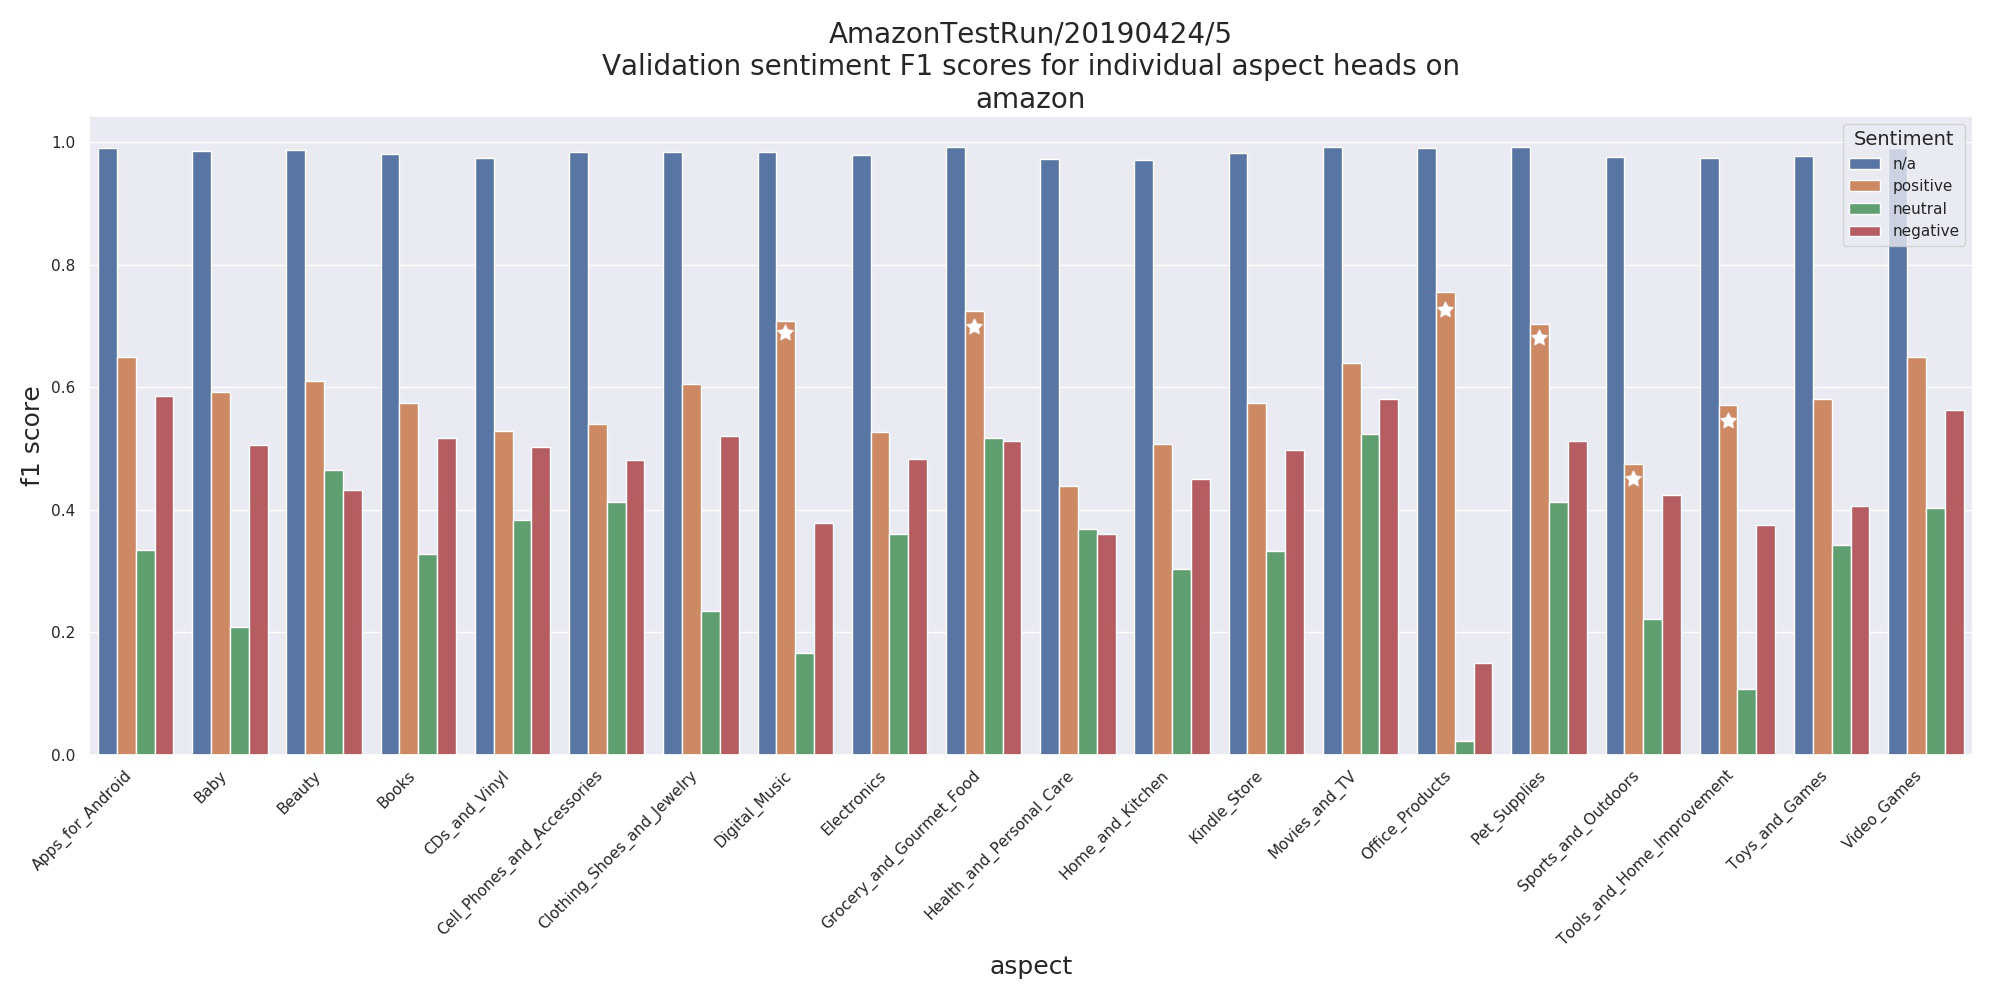
\includegraphics[width=\textwidth]{figures/06_results/06_am_final_val_f1Sent}
    \caption{Individual aspect head micro F1 scores achieved on the validation set of the custom Amazon reviews dataset. For each aspect head, this figure reports the F1 score split by the sentiment class as well as the n/a label. Aspects which have more positive reviews to keep the aspects balanced are annotated with a white star. Those include Digital Music, Grocery and Gourmet Food, Office Products, Sports and Outdoors as well as Tools and Home Improvement}
    \label{fig:06_am_val_f1sent}
\end{figure}

Even though no hyperparameter tuning was used the model achieved a final micro F1-score of 0.513 which is reported in table~\ref{tab:06_resultsAmazonFull}. Since this is a custom dataset, it is not possible to compare results with other architectures. However, there are two interesting elements of the result:
\medskip

\subsubsection*{Data Imbalance}
Even though the dataset is fairly balanced the results for the individual aspects are very different. Figure~\ref{fig:08_am_val_f1} in the appendix presents the F1 score for the individual aspects. Aspects, which are not balanced across the sentiment dimension {(they do not have an equal number of negative, neutral, positive reviews)} are marked as red. It is immediately obvious that the top-3 aspects with the highest overall score are red. Furthermore, the only aspect which does not have 60,000 reviews is also the aspect with the highest mean micro f1 score. 
\smallskip

The reason for this is the way aspects are balanced. If there are not enough reviews for the different sentiment categories, the missing reviews are taken from sentiment categories which have enough data. Table~\ref{tab:05_amazonDatasetStats} reports that the "Office Products" category contains more than 15 times more samples than the negative sentiment category. Therefore, the model can achieve a good F1 score by predicting a positive sentiment most of the time.
\smallskip

This behavior seems to point to the fact that the \gls{absat} architecture is very sensible to data imbalance.


It does not come as a surprise that the "n/a" label achieves the highest scores since this label naturally makes up a vast majority of the samples, but it is interesting, that the sentiment scores are that different.

\subsubsection*{Difficulty Classifying Different Sentiment Classes}

Figure~\ref{fig:06_am_val_f1sent} reports the micro F1 score for the individual sentiment classes. It should be noted that even classes which contain the same number of positive, negative and neutral reviews like "Books" for example achieve different results for the sentiment classes. Usually, the positive class achieves the highest score, negative comes second and neutral is generally last. There are two possible explanations for this phenomenon.
\smallskip

It may be possible to explain this behavior by looking at the overall model instead of just individual aspect heads. In total, there are more positive aspects than negative or neutral reviews. Even though the transformer base should focus on general sentence understanding, the model will be skewed towards more positive reviews. In other words, the transformer gives positive reviews more attention than negative reviews. Therefore, it is easier for the aspect heads to predict a positive sentiment than a negative sentiment, even though the balanced heads do not have any advantage by predicting more positive sentiment.
\bigskip

Another possible explanation might be that it is just easier to predict positive and negative reviews than a neutral sentiment polarity. Customers usually, review a product if they are either very happy or very unhappy. When they like or dislike a product, they use phrases which are easier to assign a positive or negative sentiment. However, the reason for giving a product a neutral review is more nuanced than a strong positive or negative emotion. In fact, neutral reviews often contain reasons which are both positive and negative. This differentiation is very challenging for a classifier. 
\smallskip

The nature of neutral product reviews is also very different than a neutral sentiment polarity in the GermEval-2017 and the Organic-2019 datasets. In those instances, a neutral sentiment usually means that the aspect was mentioned but neither positively or negatively. This is different compared to a review where a customer weights the advantages and disadvantages of product or service.

\subsubsection*{Hyperparameter Tuning}
\label{sec:06_hpTuningAmazon}
As already mentioned, we did not perform any hyperparameter tuning on this dataset. This lack of tuning is very noticeable when looking at the reported F1 score for the test and dev splits. Usually, the result for the dev portion of the data is much higher because this part is typically used for hyperparameter optimization. Therefore, researches pick the model with the highest score on the dev split, indirectly picking a model which is overfitted on the validation split to an extent. This result demonstrates that it is important never to perform optimization on the test split. However, if no optimization is performed at all, the validation split can be used as additional data for the training.  



\subsection{Results for Organic-2019}
\label{sec:06_ResultsOrganic}

Organic-2019 is a dataset on organic food which was labeled by the social computing group at \gls{tum} at the beginning of 2019. It contains 10,439 sentences which are annotated with "entities" and "aspects". Each sentence classified as "domain-relevant" receives an entity class. This entity class is further annotated with an attribute class. The sentiment is then annotated for this specific entity-attribute combination.
\medskip

There are 9 entities and 14 aspects which create 126 possible entity-attribute combinations. Samples exist for 114 out of the 125 possible combinations. This amount of classes means a classifier has to predict the probabilities for 456 class labels {($114*4$)} for each sentence. The appendix contains a list of all entity-attribute combinations at~\ref{li:08_og_aspects}.
\medskip

Classifiers {(and humans)} struggle with the number of fine-grained aspects. To provide an easier baseline, we created a coarse-grained version of the dataset which combines certain entities and attributes which are closely related to a total of 18 different aspects. A complete list of these aspects is located in the appendix at list~\ref{li:08_og_aspectsCoarse}.
\medskip

\begin{table}[htb]
    \centering
    \begin{tabular*}{\textwidth}{l@{\extracolsep{\fill}}rcc@{}}
    \toprule
    Variant          & \textbf{Num Aspects} & \multicolumn{2}{c}{\textbf{Micro F1}}       \\ 
    \midrule
                    &                          &\textit{dev}        & \textit{test}             \\
    \midrule

    Entity-Attributes + Sentiment   & 114    &  0.068            &   0.060                \\ 
    Entities + Sentiment             & 9        &  0.204            &   0.164               \\ 
    Entities 2C + Sentiment            & 9        &  0.152            &   0.147               \\ 
    Attributes + Sentiment            & 14        &  0.189             &   0.139               \\ 
    Coarse + Sentiment                & 18     &  0.314            &   0.255               \\ 
    \bottomrule
    \multicolumn{4}{c}{\textbf{Organic-2019 -- Dataset Partitions}} \\
    \end{tabular*}
    \caption{Report of results on different data partitions on the Organic-2019 dataset. Entity-Attributes denotes the full fine-grained combinations of entities and attributes. Entities 2C corresponds to the sentence combination technique explained in Section~\ref{sec:05_sentenceCombination}}
    \label{tab:06_resultsOrganic1}
\end{table}

Table~\ref{tab:06_resultsOrganic1} reports the classifier result on the data partitions. The first result corresponds to a \gls{absa} on the full set of entity-attributes combinations. 

The second row combines all attribute classes into their entity pair so that a classifier only has to predict the entity -- sentiment pair. The next row also uses entities as the classification target, but in addition, we apply the sentence combination technique. For every sentence sample, this technique combines $n=2$ sentences intending to provide context from previous sentences.

Finally, the last two rows report the results on just attribute sentiment analysis and the result on the coarse-grained data partition.
\bigskip

We used the same network architecture for each test run regardless of the data split. It consists of two encoder blocks and two aspect heads in each block. It uses a pointwise inner layer size 129 and GloVe embeddings. It is trained with a batch size of 64 and uses a linear mean head. We preprocess the data by removing stop words. The spell checker, however, is turned off.

Furthermore, we apply a dropout of 0.28 for the dropout layers in the transformer and a 0.4 dropout for the output layers. This architecture was discovered by performing hyperparameter tuning on the dataset for the coarse partition.
\bigskip

This approach has one interesting consequence. When comparing the results of the dev and test splits it is noticeable that the performance on the dev split for the coarse organic partition is significantly better. This is the phenomenon mentioned in Section~\ref{sec:06_hpTuningAmazon}.
\smallskip

However, this is not the case for the other partitions even though the data is precisely the same and the task is very similar. This aspect seems to confirm that by choosing an architecture for a task it is also possible to overfit the model architecture on this specific task.


\subsubsection*{Results for Organic-2019 Coarse}
The following section takes a more in-depth look into the dataset by utilizing the coarse data partition.

\begin{figure}[htb]
    \centering
    \subfloat[Coarse -- TEST]{
        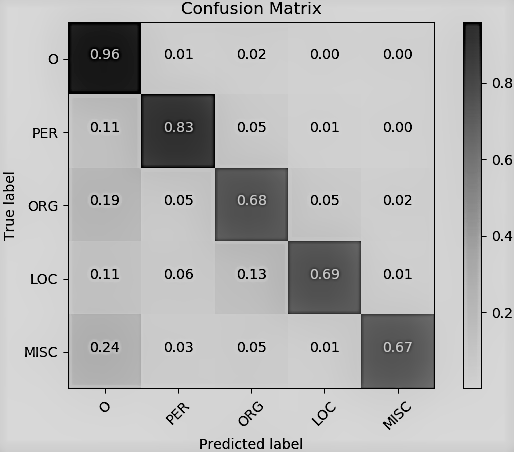
\includegraphics[width=0.49\textwidth]{figures/06_results/06_org_coarse_final_test_c_matrix}
    }
    \subfloat[Coarse -- DEV]{
        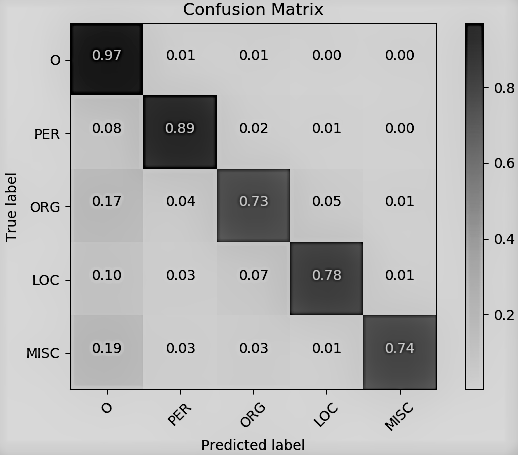
\includegraphics[width=0.49\textwidth]{figures/06_results/06_org_coarse_final_valid_c_matrix}
    }
    
    \caption{\textbf{Normalized confusion matrices for the coarse partition on the Organic-2019 dataset.} The matrix on the left {(a)} shows the performance of the model on the test set while the right {(b)} confusion matrix visualizes the performance on the validation / development set.}
    \label{fig:06_ORG_coarse_cmatrices}
\end{figure}

\bigskip
Table~\ref{tab:06_resultsOrganic2} reports on the performance of different architectures on the coarse data partition of the organic dataset. We tested four versions of the model which are the two choices for the aspect head and the embeddings. In addition, we used a random classifier as a baseline model.
\medskip

Contrary to the results on the GermEval dataset, the \acrfull{cnnh} performed significantly better than the \acrfull{lmh}. While the organic dataset contains sentence-wise annotations, GermEval provides document annotations. This main difference might point to the conclusion that the mean is more useful for long documents whereas capturing the exact sequence of words is more important for shorter sequences like single sentences for instance. 
\bigskip

\begin{table}[htb]
    \centering
    \begin{tabular*}{\textwidth}{l@{\extracolsep{\fill}}cccc@{}}
    \toprule
    Variant          & \multicolumn{2}{c}{\textbf{Macro F1}}     & \multicolumn{2}{c}{\textbf{Micro F1}}       \\ 
    \midrule
                     & \textit{dev}          & \textit{test}         & \textit{dev}              & \textit{test}         \\
    \midrule

    Random Classifier                  &  0.026         & 0.033&  0.034 &   0.038                  \\
    \gls{absat} + \gls{lmh} + FT    & 0.089     & 0.269    &  0.086 &   0.200               \\ 
    \gls{absat} + \gls{lmh} + GL    & 0.996     & 0.093    &  0.259 &   0.197               \\ 

    \gls{absat} + \gls{cnnh} + GL   & 0.113     & 0.084    & 0.341   &  \textbf{0.255}                 \\     
    \gls{absat} + \gls{cnnh} + FT   & 0.104     & \textbf{0.098} & 0.314  &   0.233                \\ 
    \bottomrule
    \multicolumn{5}{c}{\textbf{Organic-2019 -- Coarse}} \\
    \end{tabular*}
    \caption{Evaluation and comparison of \acrfull{lmh} against \acrfull{cnnh} and two embedding choices FastText {(FT)} against GloVe {(GL)} on the Organic-2019 coarse data partition.}
    \label{tab:06_resultsOrganic2}
\end{table}

When comparing the results on the organic dataset and the GermEval dataset one might wonder why the performance on the coarse organic dataset is worse compared to the GermEval dataset even though both datasets use about the same number of aspects. One might argue that GermEval provides more data and, therefore, training is more successful.

However, the number of aspects for the entity and attributes data partition is lower than the number of aspects for GermEval and their performance is even worse.

This aspect points to issues regarding the dataset and a potentially more difficult task. 
\medskip

The total amount of samples in the organic dataset is about half of the GermEval dataset. However, in practice, there are far more domain-irrelevant sentences in the organic dataset than in GermEval. Since these sentences do not contribute useful information for \gls{absa} models, we can not take advantage of this data. Consequently, the organic dataset is even smaller than the GermEval dataset when discarding the domain irrelevant sentences.
\medskip

The version of the organic dataset we used for the evaluation contained many samples with encoding issues. Since GermEval uses document annotations, it is not as problematic when some words cannot be encoded. However, when a sentence only contains a few words, it is imperative to get all words to be able to understand the sentence. 

It is important to note, however, that future versions of the organic dataset do not contain encoding issues anymore.
\medskip

Another factor are the aspects themselves. GermEval uses aspects which can be differentiated easily. The aspect of \textit{buying a ticket} {((Ticketkauf))} is very different to the aspect "\textit{train ride}" {(Zugfahrt)}. The organic dataset uses aspects which are hard to differentiate, even for human annotators because some of them are very similar.
\medskip

Previous experiments show that the \gls{absat} model has issues with imbalanced datasets. Especially for the fine-grained version which contains all entity-attribute combinations, there are some aspects which are quite common and others where only one sample exists.
\medskip

Finally, it is possible that the chosen architecture is not the optimal choice for a sentence annotated dataset. The chosen \gls{absat} architecture relies on a 1:1 sentence-label relationship. This relationship means that for every sample it needs zero or more unique class labels. This is an issue for sentence annotations because one the one hand we need context from previous sentences while on the other hand, we can not classify multiple sentences at the same time.
\smallskip

It is possible to classify documents but only if the document has unique labels. This means the transformer is capable of classifying a document with multiple sentences with aspects A, B and C. However, the \gls{absat} model cannot classify two sentences at the same time when both sentences are the same aspect.
\medskip

We tried to overcome this limitation by prepending previous sentences to the current sentence. Hence, only classifying the current sentence and thereby circumventing the limitations. However, as table~\ref{tab:06_resultsOrganic1} shows this approach hurts the performance.
\section{Impact of Multitask Learning}
\label{sec:06_ResultsMultitask}

As explained in Section~\ref{sec:04_multitask} we test the effect of \acrfull{mtl} by predicting an additional sentiment label on the GermEval dataset.

Table~\ref{tab:06_resultsMultitask} shows the performance of the transformer with- and without the additional task.  

\begin{table}[htb]
    \centering
    \begin{tabular*}{\textwidth}{l@{\extracolsep{\fill}}cccc@{}}
    \toprule
    Variant          & \multicolumn{2}{c}{\textbf{Macro F1}}     & \multicolumn{2}{c}{\textbf{Micro F1}}       \\ 
    \midrule
                     & \textit{dev}          & \textit{synchronic test}         & \textit{dev}              & \textit{synchronic test}        \\
    \midrule
    \gls{absat} + \gls{lmh} + FT                   & 0.150     & 0.117    &  \textbf{0.458}   &   0.390        \\ 
    \gls{absat} + \gls{lmh} + FT + \gls{mtl}       & 0.135   & 0.120 &  0.453   &   \textbf{0.398}    \\ 

    \bottomrule
    \multicolumn{5}{c}{\textbf{GermEval-2017 Dataset -- Multitask}} \\
    \end{tabular*}
    \caption{\textbf{Results for \acrfull{mtl} on GermEval-2017.} The \gls{mtl} model is trained with the additional task of detecting the overall sentiment for a task. This auxiliary task does not count into the calculation of the F1 score.}
    \label{tab:06_resultsMultitask}
\end{table}

With the additional task, the model performance improved slightly. The baseline system achieved an F1 score of 0.390 whereas the \gls{mtl}-version achieved 0.398. While this is a very small improvement over the baseline, this increase in performance is achieved without adding any new data.
\medskip

This specific task has data points for every sample whereas there is usually just one aspect per sample. By adding this task, the gradient flow through the transformer base is doubled. Even if a sample has two aspects, we still increase the gradient flow by 33\%.


\section{Impact of Transfer Learning}
\label{sec:06_ResultsTransfer}

Finally, we discuss the results of the transfer learning experiments. As discussed in~\ref{sec:04_transferLearning} we use the Amazon reviews dataset as a big source dataset. This dataset contains 1,193,258 reviews across 20 aspects. In this experiment, we try to transfer this knowledge from the Amazon reviews domain to the organic dataset domain.
\medskip

For this experiment, we have to use the same architecture for both systems to be able to train on both. Since we want to improve upon our target domain, we use the same configuration as for the experiments on the coarse organic data partition. The only difference is that we limit the vocabulary size to 40,000. As a consequence of this limitation, uncommon words are replaced by "<UNK>". Therefore, it is not possible to compare the performance reported in table~\ref{tab:06_resultsOrganic2} directly with these results. 

To still compare the performance, we also trained the same architecture with the same vocabulary restrictions without the knowledge transfer as a baseline.
\medskip

\begin{table}[htb]
    \centering
    \begin{tabular*}{\textwidth}{l@{\extracolsep{\fill}}cccc@{}}
    \toprule
    Variant          & \multicolumn{2}{c}{\textbf{Macro F1}}     & \multicolumn{2}{c}{\textbf{Micro F1}}       \\ 
    \midrule
                                                 & \textit{dev}          & \textit{test}         & \textit{dev}              & \textit{test}        \\
    \midrule
    \gls{absat} + \gls{lmh} + FT                   & 0.083     & 0.084    &  0.240    &  0.197        \\ 
    \gls{absat} + \gls{lmh} + FT + \gls{tl}       & 0.084     & \textbf{0.116}    &  0.298    & \textbf{0.269}        \\ 

    \bottomrule
    \multicolumn{5}{c}{\textbf{Amazon reviews > Organic coarse -- Transfer Learning}} \\
    \end{tabular*}
    \caption{\textbf{Impact of \acrfull{tl} on the model performance.} The transformer was first trained for five epochs on the amazon reviews dataset. After this, the aspect heads were exchanged for the new task on the organic-2019 coarse data partition. For this experiment we reduced the combined vocabulary size to the 40,000 most frequent words. Therefore, it is not possible to directly compare the performance of these results to the results reported in table~\ref{tab:06_resultsOrganic2}. To proof wether or not \gls{tl} can boost performance we also trained a non-\gls{tl} baseline which uses the same vocabulary as the \gls{tl} version.}
    \label{tab:06_resultsTransferLearning}
\end{table}

\begin{figure}[htb]
    \centering
    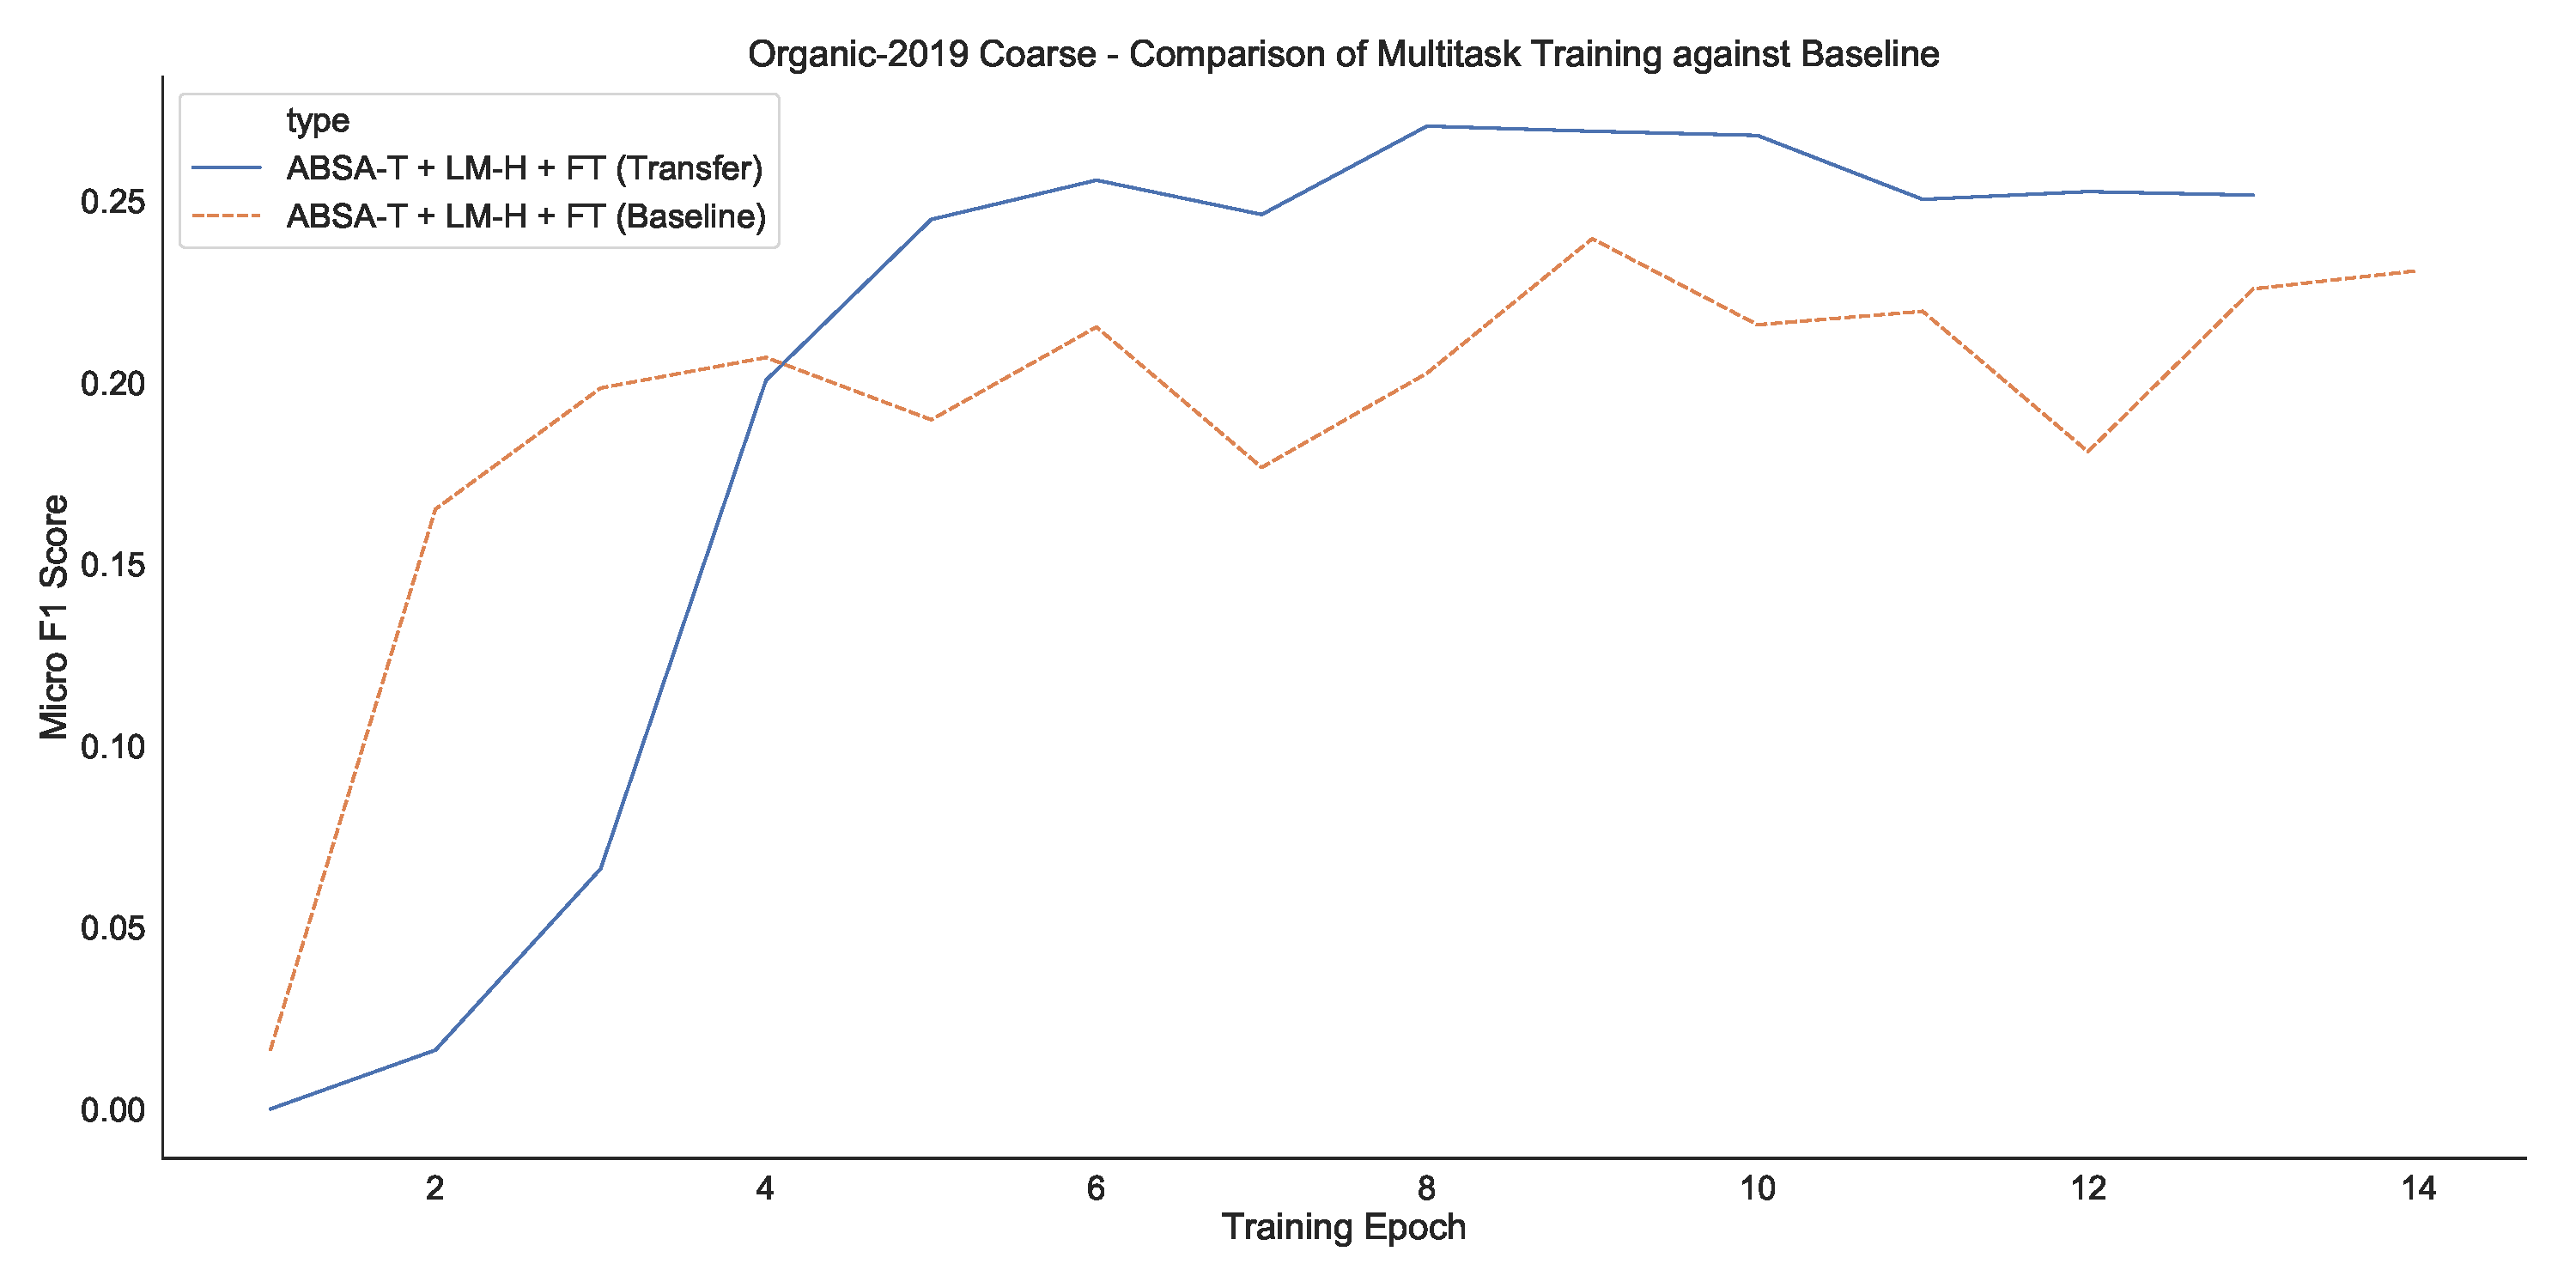
\includegraphics[width=\textwidth]{figures/06_results/06_org_coarse_transfer}
    \caption{\textbf{Performance comparison of a model using transfer learning {(blue)} against a baseline model {(orange)}.} The transfer learning model was trained on the amazon reviews dataset as the source dataset. After 5 epochs of training on the amazon dataset normal training on the coarse organic dataset started,}
    \label{fig:06_org_coarse_transfer}
\end{figure}


Table~\ref{tab:06_resultsTransferLearning} reports the results for the transfer learning experiment. The baseline is reported in the first row while the second row shows the result of the transfer learning experiment. 
\medskip

As reported, the model which was pre-trained on the Amazon reviews dataset performed significantly better than the baseline. The baseline achieved a micro F1 score of 0.197 while the \gls{tl} achieved a 35.5\% increase in performance. 
\medskip

Figure~\ref{fig:06_org_coarse_transfer} visualizes the training process by plotting the F1 score during target training of the baseline and the \gls{tl}-model. The baseline model started reasonably strong up until the fourth epoch where the transfer learning approach overtakes it. It seems as if the \gls{tl}-model is too domain-specific at first and is not able to produce any meaningful data for the transformer heads.
\medskip

It takes roughly three epochs until the \gls{tl}-model can overcome this issue. The reason for this is the unique learning scheduler that the transformer uses. The learning rate starts very low and increases linearly during a warmup phase. After the warmup phase the scheduler reduces the learning rate again.
\medskip

In the beginning, the learning rate is too low to make an impact on the pre-trained weights. However, when the learning rate starts increasing the optimizer can change those pre-trained weights which put the emphasis on the wrong, domain-specific aspects. This is the point where the F1 score drastically improves because the model is able to take full advantage of the pre-training.